\documentclass[11pt,a4paper]{report}
\usepackage[utf8]{inputenc}
\usepackage{amsmath}
\usepackage{amsfonts}
\usepackage{amssymb}
\usepackage[utf8]{inputenc}
\usepackage[T1]{fontenc}
\usepackage{textcomp}
\usepackage{gensymb}
\usepackage{graphicx}
\usepackage{float}
\begin{document}

\begin{titlepage}

\newcommand{\HRule}{\rule{\linewidth}{0.5mm}} % Defines a new command for the horizontal lines, change thickness here

\center % Center everything on the page
 
%----------------------------------------------------------------------------------------
%	HEADING SECTIONS
%----------------------------------------------------------------------------------------

\textsc{\LARGE Utrecht University}\\[1.5cm] % Name of your university/college
\textsc{\Large Master Thesis Project}\\[0.5cm] % Major heading such as course name
%\textsc{\large Minor Heading}\\[0.5cm] % Minor heading such as course title

%----------------------------------------------------------------------------------------
%	TITLE SECTION
%----------------------------------------------------------------------------------------

\HRule \\[0.4cm]
{ \huge \bfseries Hair Rendering: Importance Sampling of Dual Scattering Approximation}\\[0.4cm] % Title of your document
\HRule \\[1.5cm]
 
%----------------------------------------------------------------------------------------
%	AUTHOR SECTION
%----------------------------------------------------------------------------------------

\begin{minipage}{0.4\textwidth}
\begin{flushleft} \large
\emph{Author:}\\
Jeffrey \textsc{Lemein}% Your name
\end{flushleft}
\end{minipage}
~
\begin{minipage}{0.4\textwidth}
\begin{flushright} \large
\emph{Supervisor:} \\
Prof. Remco \textsc{Veltkamp} \\ % Supervisor's Name
%Dr. Robby T. \textsc{Tan} \\ % Supervisor's Name
%Desmond \textsc{Chik} \\ % Supervisor's Name \\
%Daniel \textsc{Heckenberg}  % Supervisor's Name \\
\end{flushright}
\end{minipage}\\[4cm]

% If you don't want a supervisor, uncomment the two lines below and remove the section above
%\Large \emph{Author:}\\
%John \textsc{Smith}\\[3cm] % Your name

%----------------------------------------------------------------------------------------
%	DATE SECTION
%----------------------------------------------------------------------------------------

{\large \today}\\[3cm] % Date, change the \today to a set date if you want to be precise

%----------------------------------------------------------------------------------------
%	LOGO SECTION
%----------------------------------------------------------------------------------------

%\includegraphics{Logo}\\[1cm] % Include a department/university logo - this will require the graphicx package
 
%----------------------------------------------------------------------------------------

\vfill % Fill the rest of the page with whitespace

\end{titlepage}

%----------------------------------------------------------------------------
% Standard thesis layout:
%
% 1. Title page: including student name, student number, supervisor names, and date
% 2. Abstract
% 3. Acknowledgement (optional)
% 4. Chapter 1: Introduction
% 5. Chapter 2: Related work / Background Knowledge
% 6. Chapter 3: Theory
% 7. Chapter 4: Experimental Results and Evaluation
% 8. Chapter 5: Conclusion
% 9. Appendix (optional)
% 10. References
%
\begin{abstract}

Rendering human hair models using individual hair fibers is a challenging task. It is challenging because of the extensive amount of hair fibers required to render a realistic model. Moreover hair fibers are very thin, resulting in noise in the renderings. To reduce this noise in a physically accurate way, more samples need to be taken. Marschner et al. (2003) proposed a physically based single fiber scattering model to render realistic human hair fibers. It is considered the founding work of current approach to physically based rendering human hair fibers.
%~\cite{marschner}

%~\cite{zinke}
When rendering light colored hair, multiple fiber scattering is essential for the appearance of the hair color. Zinke et al. (2008) extended the work of Marschner by splitting multiple scattering up into two components: global multiple scattering and local multiple scattering. Global multiple scattering approximates the multiple scattering contribution, thereby reducing the rendering time considerably. Local multiple scattering resembles the Marschner model to keep the single fiber scattering characteristics. This approach is known as the dual-scattering method. 

%~\cite{eon2013}
Importance sampling is a widely used noise-reduction technique to speed up renderings. By applying importance sampling, samples are not taken randomly (as is the case for uniform sampling), but are sampled according to a probability density distribution that favors samples that contribute more to the output rendering. This reduces noise faster and thus reduces the amount of samples that are required to produce noise-free renderings. Both uniform and importance sampling should eventually converge to the same result, with importance sampling reaching it faster.

%~\cite{eon2013}
d'Eon et al. (2013) proposed an importance sampling strategy that works particularly well for the Marschner model. This importance sampling strategy can also be applied to the dual scattering method. It is therefore very interesting to evaluate whether applying importance sampling to the dual-scattering method reduces the noise as well. This forms the main goal of this thesis: to find out if multiple importance sampling applied to the dual scattering method leads to a significant reduction of noise in the rendered image.

This report concludes by measurement and visual inspection that importance sampling for the dual-scattering method does not significantly increase the quality of the renderings compared to uniform sampling. Such a small increase in quality is not what was expected. A possible explanation is that the effect of multiple scattering is less dependent on specific sampling directions. It essentially smoothens the contribution from any direction and therefore, importance sampling does not significantly outperform uniform sampling.

\end{abstract}

\tableofcontents

\chapter{Introduction}

% a. State the background of the field, why it is interesting, what the possible applications are.

Hair rendering has always been a challenging task due to the amount of hair strands and the complex scattering behaviour between them. A human head may consist of over 100.000 hair strands and rendering them in a realistic and efficient way is challenging. Furry animals may even consist of over millions of hair strands. It is easy to see that the amount of strands provides us with a big challenge. Efficient rendering models should be devised.\\

Hair rendering becomes more important as more physically accurate models are constructed. The following industries benefit from realistic looking hair models:

\begin{itemize}
\item Animation movie industry: to efficiently render realistic hair, instead of simplified models.
\item Game industry: to enhance realism and for better visual effects.
\item Clothes manufacturers: to be able to realistically render custom fabrics and see what the visual appearance of the fiber structure will look like under different lighting conditions.
\item Hair styling industry: to realistically render the appearance of hair styling products applied to the hair.
\end{itemize}

Since rendering individual fibers is very time consuming, a lot of work has been put into approximating the appearance of a hair volume. For example, by applying transparent textures to a bounding volume to give the illusion of a realistically looking hair model. This approach may work well for a still image or for applications that do not focus on hair so much, but is not very flexible for movie or game industries. These industries often have dynamic environments in which hair might be animated or lights may change position, leading to shifting highlights that are more difficult to manage using non-physical based approaches.

Nowadays, improved hardware makes it possible to render models of individual fibers. This opens the door to physically based models based on ray-tracing. Path-tracing is the most realistic way of rendering the fibers by considering all the scattering events between light rays and individual fibers and consequently adding up the contributions along the way. It still takes up a substantial amount of time to render a single frame. The time is heavily dependent on the amount of hair fibers, but to overcome the hundred of thousands of hair strands, efficient rendering models should be devised.


\section{Goal and approach}

The work in this thesis is primarily concerned around the work of three publications. It starts with the Marschner model proposed by Marschner et al.~\cite{marschner} which forms the foundation of hair rendering in this thesis. The dual scattering model by Zinke et al.~\cite{zinke} extends the Marschner model with an efficient strategy to render volumes of hair. The third work is the importance sampling strategy devised by d'Eon et al.~\cite{eon2013}.

\subsection*{Goals}
% b. State your goal (what problems you really want to solve)

The main goal of this thesis is to find out if multiple importance sampling applied to the dual scattering method leads to a significant reduction of noise in the rendered image. We try to achieve this by extending the dual scattering model from Zinke et al.~\cite{zinke} with the importance sampling strategy proposed by d'Eon et al.~\cite{eon2013}. Importance sampling is a variance reduction technique that works very well together with Monte-Carlo integration. The focus will be on the importance sampling strategy. There are in general two problems that need to be tackled.

\begin{itemize}

\item[1] The method in this report is based on the traditional Marschner model, which is not strictly energy conserving. The improved approach by d'Eon et al.~\cite{eon2011} fixes the shortcomings and they also provided an importance sampling method in their follow up paper~\cite{eon2013}. This importance sampling strategy is used in this report to importance sample the dual scattering method. Since the dual scattering method is based on the "flawed" Marschner model, this can lead to a slightly darker or lighter image. The goal is to see whether the results are still acceptable.

\item[2] A second problem is the global illumination computation, given a direction through the hair volume. There are different ways to gather this and in this report a  voxel grid is used to store the density of the hair model at specific locations in three-dimensional space. This provides some issues with aliasing at edges of voxel cells, that need to be solved.

\end{itemize}

The ultimate goal is to see whether the importance sampling method proposed by d'Eon et al.~\cite{eon2013} can be used efficiently for the dual scattering approximation model by Zinke et al.~\cite{zinke} and thereby speed up the rendering time.

\subsection*{Approach}
% e. State how you want to approach the problem

To evaluate the importance sampling strategy, rendering results are generated to visually compare results obtained by using uniform sampling with the results obtained by using importance sampling. This gives a gut feeling about the efficiency of the sampling strategy. Additionally I will vary the number of samples per pixel to compare the same output renderings, with the only difference in increasing numbers of samples per pixel. This evaluation is done by computing the variance between these images.

Moreover, the variance of the produced renderings are compared with the ground truth. Setting the ground truth to a real-world hair model is not practical, because a real world hair model is too complex to accurately model in modeling software. Think about the hair orientations, pigment changes along the hair strand and hair cut in general. Instead, the ground truth is set to the results obtained by using 512 samples with uniform sampling.\\

The rest of this report is divided into a background section, where the basics are explained regarding radiometry and hair rendering. Related work explains the different methods that exist to render hair. Here the Marschner model and the Dual Scattering approximation model are explained in depth, because these models are the basis for the work in this thesis. Additionally, an importance sampling strategy for physically based hair fiber models is explained from d'Eon at al.~\cite{eon2013}. After the related work, we explain the approach on how to implement the dual scattering approximation with with multiple important sampling. After that we compare renderings from uniform sampling and importance sampling by looking at the variance. After that, the results are presented showing the efficiency and the analysis of the importance sampling function versus the uniform sampling version of the dual scattering approximation model.

%
% ===============================================================================
%

\chapter{Background}

Hair comes in different styles. According to Ward et al.~\cite{ward} hair can be smooth, jagged, wavy or curly depending on the ethnic group. Three different ethnic groups are distinguished: Asian, African and Caucasian hair. A hair fiber can either have a circular or elliptical cross section. Asian hair tends to be very smooth and regular with a circular cross section, whereas African hair is very irregular and has an elliptical cross section. Caucasian hair is inbetween and can be a mixture of both properties.

The follicle is the active part of hair under the skin and produces keratin proteins that compose the hair material~\cite{hadap}. The visible part of the hair is called the hair shaft. Hair has an almost uniform cross section, natural twist and natural curvatures all along~\cite{hadap}. It makes the hair appear curly, straight, fuzzy, smooth, etcetera. These parameters are characteristic for the ethnic group.

A hair fiber of the human scalp consist of three layers. The outside layer is the cuticle. The cuticle is a thin sheath of protective layers that surround the inner cortex. It forms the interface between the fiber and the air. The protective sheath consist of flat cells on top of each other. Because of the overlapped arrangement the surface normal is tilted slightly from the overall normal of the fiber's surface. According to Marschner et al.~\cite{marschner} the surface normals are tiled by approximately 3 degrees toward the root. See figure~\ref{fig_hair_structure} for a view on the cuticle scales.

The center of the hair fiber consists of the medulla: a pigmented core. The pigments give hair its color. The cortex is the core of the fiber and provides the strength for the hair fiber. The cortex is filled with keratin, contributing 90\% of the total weight~\cite{ward}. Keratin is a stiff material that causes hair to be easily bend and twisted, but hard to shear and stretch.

Hair consists of amorphous proteins that act as a transparent medium with an index of refraction of $\eta = 1.55$~\cite{ward}. A hair model will later be introduced that models hair fibers as dielectric cylinders where the index of refraction is important in deciding the refraction angle and the amount of Fresnel reflection.




\begin{figure}[h]
\begin{center}
\begin{tabular}{cc}
\includegraphics[scale=0.3]{images/hair_structure.jpeg} & \includegraphics[scale=0.27]{hair-core.png} \\
\end{tabular}
%\includegraphics[scale=0.4]{images/hair_structure.jpeg}
\caption{On the left the tilted cuticle scales on the outside of the hair fiber (taken from Marschner et al.~\cite{marschner}). On the right a cross section overview of the core of a hair fiber, consisting of the cuticle scales with the cortex and medulla (taken from Morganti~\cite{morganti2015}).}
\label{fig_hair_structure}
\end{center}
\end{figure}


\section{Rendering hair}

Marschner et al.~\cite{marschner} explain that hair rendering is a complex task, because local and global properties of hair must be taken into account. Local properties describe how light interacts with hair fibers and global properties describe the propagation of light through a volume of hair. In general, hair can be modelled explicitly or implicitly.

\subsection{Explicit representation}

Hair rendering research began by analyzing hair models using an explicit representation. This means that a hair model is represented as individual strands, or one-dimensional curves in three-dimensional space. Building on these foundations, researchers tried to find an efficient model to render a full head of human hair. Though several paths have been followed, modelling a full head of hair remains a challenge due to the geometric complexity and the thin nature of an individual strand coupled with the complex scattering effects and shadows that occur among the hairs~\cite{ward}.

\subsection{Implicit representation}

Implicit hair representations stay away from the complexities of individual strands. With implicit representations, hair is rendered by approximating the appearance of the several strands using simpler and more efficient rendering strategies. Voxel grids, multi-layer textures or polygonal boundary representations are some of the possibilities to efficiently render a full hair model.

Implicit hair is usually modelled as a volume or polygonal boundary representation. Implicit representations work great when looking at hair from a distance, because at a distance the detail is hardly visible. Moreover, it is much faster in rendering and still giving good-looking results.

%Kajiya and Von Herzen [] suggested that volume densities were potentially capable of rendering hair and furry surfaces. Kay et al [] tried to implement this via three-dimensional array of parameters. This means that a voxel cell can be maintained that holds data for each cell describing the average properties of the objects existing in this voxel cell.
%A hair density function can then be used to determine where the hair strands are and what the 

%Hair fibers cast shadows onto each other and they also receive or cast shadows on other objects in the scene. Self-shadowing is very important to render realistic looking hair. Without it may result in flat images. In general, there are two rendering strategies to incorporate self-shadowing in hair: ray casting through volumetric densities and shadow maps.



%Different known implicit representation

%Volumetric textures (or texels) [61], [62] avoid the aliasing problem with prefiltered shading functions [survey on hair modeling].



The downside of implicit representations is that it is not physically based and it is not flexible. Scattering behavior are usually simplified to work only for specific viewing directions. For physically based rendering, the explicit representation is the only way to go.

\subsection{Geometric complexity}
\label{sec_geometric_complexity}

A human scalp may consist of over 200.000 hair strands. Some animals, such as bears might realistically be rendered with millions of hair strands. It is clear that the amount of hair fibers lead to a geometric complex challenge. 

A hair fiber is naturally represented as a curved cylinder. For rendering, these cylinders are usually approximated to make computing intersections more efficient. There are strategies to render curves. Curves can be treated as:

\begin{itemize}
\item \textbf{Connected triangle strips} facing the camera. Triangles are easy to intersect and a strip that always faces the camera will always be intersectable.

\item \textbf{Cylindrical primitives}. This is the most realistic solution, because it comes closest to how a hair fiber is physically represented. It is similar to the previous approach, except that the normal is now adjusted to account for a cylindrical shape.

\item \textbf{Trigonal prisms}. This is an extension to camera facing triangle strips, making three ribbons and attaching the ends together to form a trigonal prism.

\item \textbf{Ribbons}, in which a triangle strip is constructed following the curvature of the three-dimensional curve. This triangle strip is not necessarily camera facing.

\end{itemize}

In this thesis the Physically Based Ray-Tracing (PBRT) framework is used. This is an open source physics based rendering framework created by Pharr et al.~\cite{pharr2017}. It is used by students to understand the theory of physically based rendering and academics to test their physics based rendering algorithms. The framework is extensively documented in their corresponding book~\cite{pharr2017}.

In PBRT hair fibers are represented as a three-dimensional curve with a certain defined width. When rendering, these curves are treated as cylinders by creating a camera facing triangle strip where the normal is adjusted to reflect a cylindrical primitive (the second option from the list above).

\subsection{Aliasing problem}

A hair fiber is extremely thin. So thin that it is much smaller than the size of a pixel. When tracing a ray through a pixel it will most likely miss the hair fiber. This results in aliasing problems. According to Hadap et al.~\cite{hadap} there are in general two strategies to perform anti-aliasing:

\begin{itemize}
\item Oversampling: With oversampling you cast a lot of rays through a single pixel so that enough rays hit the fiber to smooth out the aliasing effect. This is a very expensive solution, because it increases rendering time considerably For example, tracing 128 samples through a pixel could lead to a 128 times higher rendering time.

%First the hair fiber is projected onto the view plane. This makes it possible to accurately determine what pixels are affected by the hair fibers. By doing this for all hair fibers, we know exactly which hair fiber contributes to a certain pixel. By sorting the hair fibers for each pixel from front to back, we know what hair strand is before the other. The thing that needs 

%This results in point locations on the view plane. These points describe the exact location where the hair fiber is  Now we know what pixels are affected and their accurate positions inside the pixel.

\item Pixel Blending: blend the contribution of each hair fiber per pixel. This comes close to rasterization. Assuming that a curve is represented as a one-dimensional curve in three-dimensional space, then a fiber consists of a sequence of curve points. Drawing a spline based on these curve points, one can compute the contribution at each fragment of the curve, then backprojecting on the camera plane to find out which pixel is affected and add the contribution to the pixel. Blending needs to be performed to incorporate fibers that are positioned behind each other.

\end{itemize}

Physically based rendering is based on ray-tracing, so in this project the aliasing problem is overcome by oversampling and by giving each hair fiber a certain width when rendering. Increasing the width of a hair fiber increases the chance of being intersected. This makes it easier to ray-trace, thereby reducing the need for many samples. Different software packages have different optimizations to render curves.

\subsection{Mathematical notation}
\label{sec_mathematical_notation}

The notation that is used in this thesis is the same as the one used by Marschner et al.~\cite{marschner} and is common in the field of hair rendering. A hair strand is represented as a one-dimensional curve in three-dimensional space. A $uvw$ coordinate axis is attached to any point along the curve.

The $u$-axis is tangent to the hair fiber and pointing in the direction from the root toward the tip. $v$ and $w$ complete a right-handed orthonormal basis and are situated in the normal plane of the hair fiber. If the cross section is elliptical, then  $v$ represents the major axis and $w$ the minor axis. The direction where the illumination is coming from is denoted by $\omega_i$ and the direction in which light is scattered is $\omega_r$. These directions are expressed in spherical angles $(\theta_i, \phi_i)$ and $(\theta_r,\phi_r)$ respectively.

The longitudinal inclinations with respect to the normal plane are denoted $\theta_i$ and $\theta_r$ and are measured so that $0\degree$ is perpendicular to the hair and $90\degree$ is $u$ and $-90\degree$ is $-u$. The azimuths around the hair are denoted $\phi_i$ and $\phi_r$, measured so that $v$ is $0\degree$ and $w$ is $+90\degree$.

Derived angles are used, such as the difference angle $\theta_d = (\theta_r - \theta_i)/2$. The relative azimuth $\phi = \phi_r - \phi_i$. The half-angles are $\theta_h = (\theta_i + \theta_r)/2$ and $\phi_h = (\phi_i + \phi_r)/2$. Figure~\ref{axis_overview} shows an overview of the axes and spherical angles.

\begin{center}
\begin{figure}

\includegraphics[scale=.4]{images/axes.jpeg}

\caption{An overview of the coordinate axes and the spherical angles with respect to a hair fiber. This is the convention used in this thesis and is used by Marschner et al. and most other hair rendering algorithms. Picture taken from Marschner et al.~\cite{marschner}.}
\label{axis_overview}

\end{figure}
\end{center}

\section{Radiometry}
It is important to understand the terminology in radiometry to get a good understanding of the theory that is explained in this thesis. This section explains the radiometric quantities that are important to understand for hair rendering and rendering in general.

\subsection{Power and radiant flux}

Power is the rate at which energy is transferred and is expressed in watts (W). A single watt describes the transfer of a single Joule (J) of energy per unit time (s). All electronical devices consume power in one way or another. In terms of rendering we most often talk about power in the form of light propagating through the scene. 

Lights are emitting light particles through the scene at a certain rate. These elementary light particles are called photons. The stronger the light, the faster a light source emits photons in the scene. Photons exhibit a wave-particle duality. On one side they can be treated as minuscule particles and on the other side they can be treated as waves, or more specifically: electromagnetic waves.

The rate at which a light source sends out electromagnetic waves is called radiant flux. Radiant flux $\Phi$ is the power of electromagnetic waves and describes the transfer of radiant energy (J) per unit time (s). Radiant flux is therefore also expressed in watts (W).

\subsection{Solid angle and radiant intensity}

A two-dimensional angle can be represented in polar coordiante space by drawing two lines from the center of a circle outward. The angle is then represented as the difference in orientation between the lines (see figure~\ref{fig_solidangle}). If an object can be drawn so that the angle (if extending the lines) can fully encapsulate the object, then the object is considered to be subtended by the 2D angle. Angles are represented as degrees or radians, but radians are more convenient for mathematical purposes. 

A solid angle $\Omega$ is the equivalent to a two-dimensional angle, but solid angles work in three-dimensional space. It therefore can be visualized as drawing a cone outward from the center of a sphere. Similarly to the two-dimensional case, a three-dimensional object can be subtended by a solid angle. Note that objects of different sizes can have the same solid angle. This is possible as the bigger object is placed farther away from the center point of the sphere (see figure~\ref{fig_solidangle}).

\begin{figure}
\begin{center}
\includegraphics[scale=0.16]{solidangle.png}
\end{center}
\caption{Graphical representation of angles and solid angles. $\theta$ represents a two-dimensional angle. If the circle is considered a unit sphere, then the length of line $l$ equals $\theta$ radians and it subtends the red lines on the right. The solid angle $\Omega$ is a three-dimensional angle represented by a cone. At the unit sphere, the solid angle represents a surface area $A$. The red disks shown on the outside represents three-dimensional objects that are subtended by the solid angle $\Omega$. Larger objects can be subtended by the same solid angle as they are placed farther away from the center of the sphere. As the solid angle becomes infinitely small, we obtain a direction vector $\omega$.}
\label{fig_solidangle}
\end{figure}

A solid angle is a dimensionless unit of measurement called a steradian ($sr$). Steradian is coming from squared radian as is an obvious generalization when you realize angles are represented in radians.\\

The radiant intensity $I$ is a measure of the intensity of electromagnetic radiation. It can be seen as the energy flow divided by the solid angle in which it is transmitted. Radiant intensity is defined as radiant power per unit solid angle ($W \, sr^{-1}$).

\subsection{Irradiance}
\label{radiance_irradiance}

Formally, irradiance $E$ is defined as the amount of power of electromagnetic radiation per unit area incident to a surface. The unit for irradiance is watts per square meter ($W \cdot m^{-2}$). If the light is shining directly down on the surface area, the irradiance can be described as:

\begin{equation}
E = \frac{\Phi}{A}
\label{eq_irradiance1}
\end{equation} 

Figure~\ref{cosine_term_visualization} shows a simplified scenario of a directional light shining on a surface. Irradiance is the amount of radiant flux (or power) that is received per unit area. If we consider a rectangular bundle of light with width $w$ that hits the surface from a perpendicular direction $\omega_i$, then it is obvious to see that all the light falls into an equally sized rectangle on the surface (equation~\ref{eq_irradiance1}). The irradiance would be equal to the power (or wattage) of this bundle of light, divided by the surface area.

As the angle with the surface normal $\vec{n}$ increases, the direction from which it hits the surface $\omega_i'$ becomes smaller. As a result, the bundle of light spreads its power over a larger area and therefore the irradiance becomes smaller. As the angle becomes perpendicular to the surface normal $\vec{n}$, no light is reaching the surface anymore. The relationship between the angle of incidence $\theta_i$ on a surface and irradiance is expressed by the cosine of $\theta_i$. This relationship is known as Lambert's law (depicted in~\ref{cosine_term_visualization}) and the equation for irradiance becomes:

\begin{equation}
E = \frac{\Phi \cos \theta_i}{A}
\label{eq_irradiance2}
\end{equation}

\begin{figure}
\begin{center}
\includegraphics[scale=1.0]{images/svg/irradiance_radiance.jpg}
\caption{As the incoming light hits the surface at a larger angle, the irradiance decreases because the same amount of light will be spread over a greater surface area.}
\label{cosine_term_visualization}
\end{center}
\end{figure}


\subsection{Radiance}

Radiance $L$ measures irradiance with respect to a solid angle $\omega$ as the solid angle goes to zero. A solid angle going to zero essentially means that the cone shrinks in size to the limit of 0. In that case the solid angle becomes a direction $\omega$. In other words, radiance is defined as differential power $d\Phi$ per differential area $dA$ at a point $p$ for direction $\omega$ and can be written as~\cite{pharr2017}:

\begin{equation}
L(p, \omega) = \frac{d E_\omega(p)}{d \omega} = \frac{d\Phi\, \cos \theta}{d\omega\, dA}
\end{equation}

Radiance $L$ measures the light intensity per unit area on a surface. It measures the quantity of radiation that passes through or is emitted from a surface and falls within a given solid angle in a specified direction. Radiance is used to characterize diffuse emission. The unit of radiance is watts per steradian per square meter ($W \cdot {sr}^{-1} \cdot m^{-2}$).

A nice thing about radiance is that it remains constant along rays as long as the ray moves through a vacuum. This makes it very useful in rendering applications.

\subsection{Bidirectional reflection distribution function (BRDF)}
\label{sec_bsdf}

When a surface is lit by a light source, part of it will scatter back into the environment. The distribution at which light is scattered back is described by a bidirectional scattering distribution function (BSDF). It is named bidirectional, because the distribution is dependent on the incident and outgoing light direction. If the surface is opaque, which means there is no subsurface light transport or refraction, then the BSDF is described by surface reflection only. In that case the BSDF is called a bidirectional reflectance distribution function (BRDF). A BRDF function is denoted as $f_r(p, \omega_i, \omega_o)$ where $p$ is the surface position, $\omega_i$ is the incident light direction and $\omega_o$ the outgoing light direction.

A BRDF can be expressed as a ratio between the outgoing radiance $L_o$ in direction $\omega_o$ and an incident irradiance $E_i$ from direction $\omega_i$. Since we are dealing with a continuous flow of energy transport (there is no snapshot of light), the BRDF ratio is expressed as a differential, as shown in equation~\ref{eq_brdf}.

\begin{equation}
f_r(p, \omega_o, \omega_i) = \frac{dL_o(p, \omega_o)}{dE(p,\omega_i)} = \frac{dL_o(p, \omega_o)}{L_i(p, \omega_i) \cos \theta_i d\omega_i}
\label{eq_brdf}
\end{equation}

The rewritten form of irradiance in the equation above comes from the definition of irradiance as has been explained in section~\ref{radiance_irradiance}.

BRDF's have two important characteristics~\cite{pharr2017}:

\begin{itemize}
\item Reciprocity: the incoming and outgoing directions can be swapped and still have the same reflection behavior: $f_r(p, \omega_i, \omega_o) = f_r(p, \omega_o, \omega_i)$.
\item Energy conservation: the total amount of energy that is reflected will always be less or equal than the amount of energy that is incident to the surface.
\end{itemize}

\subsection{Bidirectional curve scattering distribution function (BCDSF)}
\label{sec_bcsdf}

As discussed in the previous section, a BRDF describes the ratio between outgoing surface radiance in direction $\omega_o$, to incident surface irradiance from a differential solid angle $\omega_i$~\cite{ward}. Fibers are usually treated as one-dimensional curves. Curves have no area and therefore, scattering from fibers need to be described in terms of the length of a fiber.

Scattering from a fiber is thus represented by a bidirectional curve scattering distribution function (BCSDF) $S(\omega_i, \omega_o)$ that describes the ratio between the outgoing curve radiance $L_o$ in direction $\omega_o$ to the incident curve irradiance $E_i$ from a differential solid angle $\omega_i$. It shares the same physical units as a BRDF, but the concept is a little different.

\begin{equation}
S(\omega_i, \omega_o) = \frac{dL_o(\omega_o)}{dE_i(\omega_i)}
\end{equation}

Curve irradiance is proportional to incoming curve radiance:

\begin{equation}
dE_i(\omega_i) = D L_i(\omega_i) \cos \theta_i d \omega_i
\end{equation}

Here $D$ denotes the diameter of the fiber. So, curve irradiance is the amount of light falling on an infinitesimal small length of curve $dl$, times the diameter of the fiber: $D dl$. Using the former equation, the scattering integral can be written as:

\begin{equation}
L_o(\omega_o) = D \int S(\omega_i, \omega_o) L_i(\omega_i) \cos \theta_i d \omega_i
\label{eq_bcsdf}
\end{equation}


\subsection{Rendering equation}

The rendering equation is an integral and formally describes the amount of radiance leaving from a position $p$ in direction $\omega_o$. The radiance consists of the emitted radiance $L_e$ plus the integral around the sphere to integrate all incoming light $L_i$ from incident direction $\omega_i$, reflecting in direction $\omega_o$, where the BSDF is denoted by $f(p, \omega_o, \omega_i)$ indicating the contribution of incident light reflected in the outgoing direction at position $p$. The cosine factor is to take into account the angle with the surface normal (see section~\ref{radiance_irradiance}).

\begin{equation}
L_o(p, \omega_o) = L_e(p, \omega_o) + \int_{\Omega} f(p, \omega_o, \omega_i)\, L_i(p, \omega_i)\, \cos \theta_i\, d\omega_i
\label{rendering_eq}
\end{equation}

Solving this equation is the key task for a computer graphics program. Hair fibers do not emit radiance and therefore the emitted radiance can be ignored in the rendering equation. Taken into account that hair fibers are represented by curves (see section~\ref{sec_bcsdf}), the curve rendering equation that will be used in this thesis is as follows.

\begin{equation}
L_o(p, \omega_o) = D \cdot \int_{\Omega} S(p, \omega_o, \omega_i)\, L_i(p, \omega_i)\, \cos \theta_i\, d\omega_i
\label{renderingEquation}
\end{equation}

By removing the position parameter $p$, we obtain the same equation as equation~\ref{eq_bcsdf}.

%
% ===============================================================================
%  Importance sampling
% ===============================================================================
%

\section{Importance sampling}
\label{basics_importance_sampling}

% The need for importance sampling

Importance sampling is a variance reduction technique. The idea is to prefer samples that have more impact on the end result (i.e. the rendering) than samples that hardly have an influence. In other words, samples with a higher impact are more important to sample from, than samples that hardly have impact. By prefering samples of important directions we are converging faster to the correct end result, thereby decreasing rendering times significantly.

\subsection{Monte-Carlo integration}
% Introduction to monte-carlo integration 

Monte-Carlo integration is a numerical integration technique. In contrast to many other integration techniques, it can evaluate an integral using random samples, where performance is irrespective of the dimensionality of the samples.

Given an integral $\int_a^b f(x) dx$ for a function $f(x)$ over the range $[a, b]$. If it is possible to find a function $F(x) = \int f(x) dx$, then we could solve the integral analytically and there would be no need for numerical integration.

In the context of physically based rendering, the integral is often too complicated to solve analytically. The Monte-Carlo integration is a relatively simple way to be able to find the expected value of the integral $E[F(x)]$. Monte-Carlo integration is doing that by taking $N$ random samples where each sample is weighted by the probability of being sampled $p(X)$. The larger the number of samples, the more accurate the result will be, eventually converging to the correct result for the integral. The following equation describes the computation of the integral $F_N$ with the Monte-Carlo estimator~\cite{pharr2017}.

\begin{equation}
F_N = \frac{1}{N} \sum_{i=1}^{N} \frac{f(X_i)}{p(X_i)}
\end{equation}

$N$ represents the number of samples taken, $X_i$ represents the $i$-th random sample and $p(X_i)$ is the probability density for sample $X_i$. If the probability density function $p(x)$ is uniform then $p(x)$ becomes a constant $\frac{1}{c}$ and can be moved to the front of the equation, resolving to the following Monte-Carlo estimator.

\begin{equation}
F_N = \frac{c}{N} \sum_{i=1}^{N} f(X_i)
\end{equation}

Integrating over a range $[a , b]$ resolves to a constant $c = b - a$ and thus it boils down to finding the average value for $f(x)$ multiplied by the range, giving the area under the surface or when integrating around a hemisphere, the solution to the rendering equation.

\subsection{Importance sampling}
\label{section_importance_sampling}
% Adding importance sampling to the fact

It becomes interesting when the probability density function $p(x)$ is not constant for all samples. By giving certain samples a higher probability and other (less important) samples a lower probability, we can converge faster to the correct result by using less samples.

The idea behind importance sampling is to draw samples from the probability distribution function (PDF). There are different techniques to draw samples from a PDF as explained in the book by Pharr et al.~\cite{pharr2017}. Possible techniques are inversion sampling, in which the normalized cumulative distribution function (CDF) is computed, then inverted and used with a uniform random variable $\xi \in (0, 1]$ to obtain a sample $X$. Other techniques are rejection sampling.
 
It is easy to see that the better the fit of the PDF with the function $f(x)$, the better the drawn samples and the faster we converge to the correct result. If $f(x) = p(x)$ we are talking about perfect importance sampling, the most ideal case. However, it is not always possible to invert $f(x)$. If we can find a PDF that is still a close fit to $f(x)$ but is possible to invert, then we still have a better sampling technique compared to uniform sampling.

Other techniques are possible as well, such as rejection sampling, which is described in detail in Pharr et al.~\cite{pharr2017}.

\subsection{Multiple importance sampling}
% Multiple importance sampling

Sometimes we end up with a function that can be written as the product of multiple functions $f(x)g(x)$, each of which has an easy to sample PDF $p_f(x)$, belonging to $f(x)$ and $p_g(x)$ for $g(x)$.

If two sampling distributions $p_f(x)$ and $p_g(x)$ are used to estimate the value of $\int f(x)g(x) dx$, you cannot just average the results by taking N samples from $p_f(x)$ and M samples from $p_g(x)$ and average the result, because variance is additive. The way to do it is by using the new Monte-Carlo estimator for multiple importance sampling (MIS) stated in~\cite{pharr2017}: 

\begin{equation}
\frac{1}{n_f} \sum_{i=1}^{n_f} \frac{f(X_i)g(X_i) w_f(X_i)}{p_f(X_i)} + 
\frac{1}{n_g} \sum_{j=1}^{n_g} \frac{f(Y_j)g(Y_j) w_g(Y_j)}{p_g(Y_j)} 
\end{equation}

where $w_f$ and $w_g$ are weighting functions.

\begin{equation}
w_s(x) = \frac{n_sp_s(x)}{\sum_i n_i p_i(x)}
\end{equation}

An example of multiple importance sampling is when rendering complex scenes with multiple objects and light sources. When light sources are very small, the chance of being sampled (as observed from a point on a surface) is likewise very small. It is easy to imagine that lots of samples are required when evaluating the BSDF for a material to remove the noise. A better approach would be to sample from the light source. If the light source is very large, for example a skydome around the scene acting as a light source, it is more efficient to sample the BSDF of the material. Multiple importance sampling takes this effect into account. By mixing samples from the BSDF of the material and from the distribution of the light source, a selection of important samples can be used to reduce noise. 
%Pharr et al.~\cite{pharr2017} presented a nice rendering showing the effect of multiple importance sampling (see figure~\ref{fig_multi_importance}).





\chapter{Related Work}

% a. Discuss the existing methods and state why they cannot solve the problems or achieve the goal entirely.
% b. Discuss other related work or knowledge that is necessary to understand the theory explained in Chapter 3.
% c. Ask yourself if the information will be sufficient if a student who is new in the field reads this chapter.





\section{Hair rendering overview}

The explicit representation of hair provides the most physically accurate results. In this thesis, explicit representations are used. As will be explained, the Marschner model is an accurate single fiber scattering model. To increase the realistic appearance of hair volumes, more fibers should be taken into account. This leads to the concept of multiple fiber scattering. Multiple fiber scattering is analogous to subsurface scattering in solid materials and therefore necessary to increase the level of realism. Ward et al.~\cite{ward} provides a good overview on the different models in hair rendering in general.

In this section, related work regarding the development of hair models is explained, followed by an in-depth treatment of the most relevant work related to the research in this thesis.


\subsection{Single fiber scattering}

Kajiya and Kay~\cite{kajiya} provided one of the first widely used hair scattering model that was designed to render fur. Fur usually refers to a  dense coat of fine and soft hair. Their idea was that fine hair geometry should not be represented with complex geometry which leads to aliasing effects, but with texels. A texel is a three-dimensional texture map intended to represent a highly complex collection of surfaces contained within a defined volume~\cite{kajiya}.

The rendering of the hair model was based on a diffuse and specular component. The diffuse component is obtained by simply integrating a Lambert surface along one half of the cylinder facing the light source. The specular component is based on the Phong model in which light is reflected at a mirror angle along the tangent. Since the normals on the cylinder point in directions perpendicular to the tangent, the reflected light forms a cone whose angle at the apex is equal to the angle of incidence~\cite{kajiya}. The Kajiya and Kay model is clearly an ad-hoc model where hair fibers are treated as opaque cylinders, limiting the realism of the model (see figure~\ref{fig_compare_kajiya}).\\

The Kajiya and Kay model lacks directionality, meaning that hairs are fully lit independent of the light direction or eye position. Goldman~\cite{goldman} was interested in reflection and transmission and increased directionality by introducing two new attenuation factors. These attenuation factors can be used to tune the relative transmissivity and reflectivity of a hair. It does this by computing a value $f_{\textsc{dir}}$ that is multiplied with the contribution of the Kajiya and Kay model.\\

Marschner et al.~\cite{marschner} improved the Kajiya and Kay model substantially by proposing the most physically based hair scattering model at that time. Their model makes two improvements to Kajiya and Kay's model: it predicts the azimuthal variation in scattered light based on the ray optics of a cylinder, and it accounts for the longitudinal separation of the highlight into surface-reflection, transmission, and internal-reflection components that emerge at different angles~\cite{hadap}. The Marschner model is described in detail in section~\ref{sec_marschner}.

\begin{figure}
\begin{center}
\includegraphics[scale=0.15]{kajiya.png}
\caption{Comparison of Kajiya and Kay model with the Marschner model. The left image represents Kajiya and Kay's model. The center image is the Marschner model and the right image represents the original real-world photographed reference. Picture taken from Marschner et al.~\cite{marschner}.}
\label{fig_compare_kajiya}
\end{center}
\end{figure}


\subsection{Multiple fiber scattering}

Ward et al.~\cite{ward} states that for light-colored hair, recent work has shown that shadowing and attenuation alone are insufficient to produce the correct appearance. For fully realistic results multiple scattering must be accounted for.

Multiple fiber scattering extends single fiber scattering to take into account the scattering effects taking place between multiple hair strands. A single fiber scattering model can be used as the basis for multiple fiber scattering. For example, if the Marschner model is the basis for single fiber scattering, then in combination with path tracing the result is obtained for multiple fiber scattering. Path tracing is a brute-force approach that gives realistic results. However, given the geometric complexity of a hair model, it is a very time and memory intensive process. More efficient models for multiple fiber scattering models should be devised.\\

Photon mapping methods can reduce per-frame rendering times from days, required for path tracing methods, to hours~\cite{ward}. Photon mapping is a practical approach for computing global illumination in complex environments. Photon mapping is introduced by Henrik Wann Jensen~\cite{jensen} and it is, in general, a two-step approach.
The first pass in the method is constructing the photon map by emitting photons from the light sources in the model and storing these in the photon map as they hit surfaces~\cite{jensen}. The collection of photons distributed in the photon map, can be seen as a rough representation for the amount of light in the scene. The second step is that this information from the photon map is used to render the scene.

For multiple scattering in hair models, Moon and Marschner~\cite{moon} developed a model using a photon mapping approach. In the first pass, particles are traced from light sources into the hair volume and followed through multiple scattering events, and their positions and directions are stored into a 5D hierarchical data structure to record the flow of particles through space~\cite{moon}. In the second pass a density estimate is performed simultaneously in position and direction to estimate the radiance arriving at a hair from a particular direction.  This photon mapping approach leads to similar results compared to path tracing, but the biggest drawback is that it requires high resolution photon maps (memory usage) and the method is not interactive.

The Dual Scattering model by Zinke et al.~\cite{zinke} is a direct extension on top of Marschner and doesn´t have the drawbacks of photon mapping approaches. The dual scattering approximation splits up the compensation in a global and a local scattering component. The global scattering component computes the amount of irradiance reaching a certain position in the hair model. The local scattering component uses the computed irradiance to compute the scattering effects in the direct neighbourhood of the position to be rendered. More in-depth theory is provided in section~\ref{sec_dualscattering}.

%
% ===============================================================================
%  Marschner Model
% ===============================================================================
%

\section{Marschner model}
\label{sec_marschner}
%
% Goal of Marschner 
%

The biggest drawback of Kajiya and Kay~\cite{kajiya} is that their scattering model is not based on physical measurements. Instead, it uses a simple ad-hoc term with a constant linear highlight. Marschner et al.~\cite{marschner} proposed a physically based scattering model for single fiber scattering. The single fiber scattering model, or Marschner model, can be considered the status quo in modern hair rendering technology. Most physics based hair rendering model in some way or another are derived from the Marschner model. Likewise, the Marschner model forms the basis for the dual scattering approximation (by Zinke et al.~\cite{zinke}). In this section the Marschner model will be discussed in detail.


\subsection{Observations}
%
% Basic observation
%
 
In order to come up with a physically based scattering model for single hair fibers, Marschner et al. devised a setup to capture the response of light scattered against a hair fiber. 

They illuminated individual hairs with a narrow beam and measured the scattered light in various directions, using a setup based on a four-axis goniometer that positioned a light source and a CCD camera at arbitrary directions from the sample~\cite{marschner}. Their measurements show a couple of distinct characteristics for human hair.

\subsubsection{Longitudinal variation (primary and secondary highlight)}
\label{sec_longitudinal_observation}

Stamm et al.~\cite{stamm1977} and Bustard and Smith~\cite{bustard1991} measured the scattering behaviour in the incidence plane. This is the 2D slice for which the hair fiber is coplanar with the source and detector. Marschner et al. did the same measurements and placed a light source under a direction of positive and negative 45 degrees with the hair fiber ($\theta_i = +/- 45\degree$). See figure~\ref{fig_longitudinal_marschner} for the measured responses.

Observations show that synthetic hair has a highlight that appears exactly at the specular direction ($\theta_r = -\theta_i$), but for real hair fibers the specular highlight is shifted toward the root of the hair fiber. This is due to the tilted cuticle scales that have a surface orientation that is shifted by approximately 6 to 8 degrees from the ideal cylinder surface normal. This highlight is the result of scattering against the surface of the hair fiber. It is called the primary specular highlight and appears as having the color of the light source.

\begin{figure}[h]
\begin{center}
\includegraphics[scale=0.35]{images/longitudinal_response.jpeg}
\caption{The scattering behaviour in the incidence plane (longitudinal scattering). For human hair the specular reflection is shifted towards the root by a few degrees. For synthetic hair no shifted highlight is visible, because synthetic hair doesn't consist of tilted cuticle scales.}
\label{fig_longitudinal_marschner}
\end{center}
\end{figure}

Another observation from figure~\ref{fig_longitudinal_marschner} is that blond hair has a coloured secondary peak. This can be seen by the red response that is slightly higher compared to the blue and red response. The secondary peak can be explained by internal scattering. Consider the hair fiber as a cylinder; when light enters the cylinder, the light will first refract, then propagates through the core of the fiber and bounces back against the other end of the fiber. When leaving the fiber, the light refracts again. This reflection and refraction behaviour causes the deviation from the primary specular highlight. During its travel, light propagated through the center of the hair fiber, where the pigments are. These pigments absorb part of the energy in different wavelengths. This is how the secondary peak obtains its color.

Furthermore, Marschner et al.~\cite{marschner} noticed that as the scattering angle increases, the secondary highlight fades out, while the primary highlight maintains more constant amplitude. Both peaks maintain approximately constant width and at glancing angles the primary highlight becomes a sharp peak that is prominent very close to the specular direction. 


\subsubsection{Azimuthal variation}


\begin{figure}[h]
\begin{center}
\includegraphics[scale=0.4]{images/azimuthal_measurement.jpeg}
\caption{Measurements of azimuthal scattering (scattering in the normal plane). The light source is shining from the right, while the hair fiber is rotated. The green ellipse is the cross section of the fiber for different measurements with increasing rotations of the fiber. Figure taken from Marschner et al.~\cite{marschner}.}
\label{fig_azimuthal_marschner}
\end{center}
\end{figure}


Azimuthal variation is measured by placing the light and detector in the plane that is perpendicular to the hair fiber: the normal plane. In figure~\ref{fig_azimuthal_marschner} plots are displayed that show the azimuthal scattering response with varying $\phi_i$ and $\phi_r$. The setup is that the light source is fixed (targeted from right to left) and the hair fiber is rotated. 

In this normal plane setup, it is clearly visible that there are two bright out-of-plane peaks. Out of plane, because the response is captured at $\theta_r = 10$ degrees, due to the tilted cuticle scales discussed before. These peaks are called glints.

Glints change considerably in brightness and position as a function of $\theta_i$,  meaning that the hair is not rotationally symmetric~\cite{marschner}. This is because the hair is eccentric and has an elliptical cross section. More generally, the evolution of the peaks as the fiber rotates appears similar to the internal reflection from a transparent elliptical cylinder~\cite{marschner}.

Figure~\ref{fig_azimuthal_marschner} also shows a strong transmission component. This is light that passes through the hair fiber and leaving on the other side of the fiber as seen from the light source. This means that the Marschner hair model takes three scattering modes into account. R stands for reflection and T for transmission:

\begin{itemize}
\item R: Specular reflection that is deviated slightly from the perfect specular direction, due to the cuticle scales.
\item TT: Transmission component that enters the fiber, propagates through it and leaves the fiber at the other end.
\item TRT: Internal reflection, that enters the fiber, scatters back and leaves again at the same side as where it entered.
\end{itemize}

More scattering modes are possible as well, such as TRRT or TRRRT. These events are ignored, because their contributions become negligible small due to loss of energy after that many reflection events. Instead, Marschner et al.~\cite{marschner} suggests to add a little diffuse color for better looking results. In figure~\ref{female_hair} an image is shown with the three scattering components clearly visible. D'Eon et al.~\cite{eon2011} generalized the Marschner model to take into account all possible scattering events, so that no energy is lost. This is mainly important for highly transmissive hair fibers, such as white hair for polar bears. For human hair-rendering this might not directly be an issue.

\begin{figure}[h]
\begin{center}
\includegraphics[scale=0.2]{images/female_marschner.jpeg}
\caption{An image from Gray et al.~\cite{gray} showing a female with brown hair. The three scattering modes: R, TT and TRT contributions are visible in the hair. Glints give hair it's characteristic texture.}
\label{female_hair}
\end{center}
\end{figure}

\subsection{Model}

There are properties that have been used in previous work on scattering from fibers (Marcuse~\cite{marcuse1974}, Adler et al.~\cite{adler1998}, Mount et al.~\cite{mount1998}):

\begin{itemize}
\item A ray that enters a dielectric cylinder at a particular angle to the axis will always exit at the same angle, regardless of the sequence of reflections and refractions it undergoes.

\item The dependence of the scattered distribution can be analysed by examining only the projection into a plane perpendicular to the hair.
\end{itemize}

Based on the observations described in the previous subsection and the theory here, Marschner et al. came up with a model that is divided into a longitudinal scattering function $M_p$ and an azimuthal scattering function $N_p$, where $p$ is the scattering mode with $p \in \{\textnormal{R}, \textnormal{TT}, \textnormal{TRT}\}$. The resulting scattering model can then be written as:

\begin{equation}
\label{marschner_model_scatterfunction}
S(\omega_i, \omega_r) = \frac{\sum_{p \in \{\textnormal{R}, \textnormal{TT}, \textnormal{TRT}\}} M_p(\theta_i, \theta_r) N_p(\eta'(\theta_d); \phi_i, \phi_r)}{\cos^2 \theta_d}
\end{equation}

$S$ depends on incoming and outgoing angles $\omega_i$ and $\omega_r$, but can be reduced to a 2D scattering function, since the scattering model makes use of derived angles $\theta_d$, $\theta_h$ and the relative difference in azimuthal angle $\phi$ (see section~\ref{sec_mathematical_notation}).

\subsubsection{Longitudinal scattering function}
\label{marschner_longitudinal_scattering_function}

Using the first property of scattering from fibers, it can be derived that the angle of incidence is the same as the angle of reflection ($\theta_i = -\theta_r$). There are two deviations that cause the reflection to not be exactly in the specular direction (see section~\ref{sec_longitudinal_observation}). First, the surface of a hair fiber is rough, causing a spread of reflected light instead of a mirror like specular reflection. Secondly, the cuticle scales of the hair fiber are tilted, causing a 6 to 8 degrees deviation from the perfect specular direction.

Marschner et al.~\cite{marschner} approximates the longitudinal scattering function $M$ by a unit-integral zero-mean gaussian function $g(\beta, x)$, where $\beta$ equals the standard deviation and $\alpha$ equals the longitudinal shift. D'Eon et al.~\cite{eon2011} observed that the Marschner model is not entirely energy conserving for several reasons. One of the reasons is that the use of the half angle $\theta_h$ doubles the reflected energy on average. Additionally the gaussian is normalized with respect to $\theta_h \in (-\infty, \infty)$, but is evaluated for $\theta_h \in [-\frac{\pi}{2}, \frac{\pi}{2}]$, thereby losing a considerable amount of energy that is present outside of the used range. The doubling of energy is easily accounted for by doubling the half angle in the Marschner longitudinal scattering function. The resulting longitudinal functions $M$ that are used for the Marschner model are thus as follows:

\begin{align}
M_{\textnormal{R}}(\theta_h) &= g(\beta_{\textnormal{R}}, 2\theta_h - \alpha_{\textnormal{R}}) \\
M_{\textnormal{TT}}(\theta_h) &= g(\beta_{\textnormal{TT}}, 2\theta_h - \alpha_{\textnormal{TT}}) \\
M_{\textnormal{TRT}}(\theta_h) &= g(\beta_{\textnormal{TRT}}, 2\theta_h - \alpha_{\textnormal{TRT}})
\end{align}

By varying the standard deviation $\beta$, the spread of the longitudinal scattering lobe can be adjusted to simulate the rough surface of hair fibers. The longitudinal shift $\alpha$ deviates the peak from the specular direction by shifting the gaussian distribution. Some typical values for $\alpha$ and $\beta$ are presentred in table~\ref{table_marschner_alpha_beta}.

\begin{table}[h]
\begin{center}
\begin{tabular}{c|l|c}
Parameter & Description & Typical value \\ \hline 
$\alpha_{\textnormal{R}}$ & Longitudinal shift for R lobe & -10\textdegree\,to -5\textdegree \\
$\alpha_{\textnormal{TT}}$ & Longitudinal shift for TT lobe & $-\alpha_{\textnormal{R}} / 2$ \\
$\alpha_{\textnormal{TRT}}$ & Longitudinal shift for TRTlobe & $-3\alpha_{\textnormal{R}} / 2$ \\
$\beta_{\textnormal{R}}$ & Longitudinal spread for R lobe & 5\textdegree\, to 10\textdegree\, \\
$\beta_{\textnormal{TT}}$ & Longitudinal spread for TT lobe & $\beta_{\textnormal{R}} / 2$ \\
$\beta_{\textnormal{TRT}}$ & Longitudinal spread for TRT lobe & $2 \beta_{\textnormal{R}}$ 
\end{tabular}
\end{center}

\caption{Typical values for parameters for the longitudinal scattering function. $alpha$ is the longitudinal shift to represent the shift of the lobe due to tilted cuticle scales. $\beta$ is the longitudinal width, representing the spread of the energy due to rough surface of hair fibers. Taken from Marschner et al.~\cite{marschner}}

\label{table_marschner_alpha_beta}
\end{table}


\subsubsection{Azimuthal scattering function}

\begin{figure}[h]
\begin{center}
\includegraphics[scale=0.2]{circularcross.png}
\end{center}
\caption{Cross section of a hair fiber showing the different scattering modes. Taken from Marschner et al.~\cite{marschner}}
\label{fig_circular_cross_section}
\end{figure}

For the azimuthal scattering component different scattering paths inside the circular cross section of the hair need to be considered. The Marschner model takes into account 3 scattering modes, the R, TT and TRT mode. Figure~\ref{fig_circular_cross_section} shows a graphical representation of a circular cross section of a hair fiber.

Scattering from a dielectric circle is well studied. Consider a parallel beam (or ray) incident to a circular cross section at an offset $h$ from the center. A parallel beam incident to the center of a circle corresponds to the root value $h = 0$. A value of $h=1$ or $h=-1$ corresponds to beams glancing the edges of the circle. Using the offset $h$ the angle of incidence $\gamma_i$ can be computed using the following equation:

\begin{eqnarray*}
\sin \gamma_i = h & \Leftrightarrow & \gamma_i = \arcsin h \\
\eta \sin \gamma_t = h & \Leftrightarrow & \gamma_t = (\arcsin h) / \eta
\end{eqnarray*}

A ray that is incident to the unit circle can be traced as it refracts and reflects through the circle. The exit angle is not only dependent on the incidence angle (or offset from the center), but also on the number of scattering events. The number of scattering events $p$ equals 1 for the reflection case, 2 for transmission (TT) and 3 for internal reflection (TRT). The exit angle can then be calculated as follows:

\begin{equation}
\label{eq_relative_azimuth_change}
\phi(p,h) = 2p \gamma_t - 2 \gamma_i + p \pi
\end{equation}

\subsubsection{Finding roots}

Consider rendering a scene using ray tracing and that a particular camera ray is incident to a hair fiber. Figure~\ref{fig_rootfinding} represents this situation. To find the contribution of radiance towards the camera (i.e. the outgoing direction $\omega_o$), all the paths that contribute to scattering in that direction should be taken into account. These incident light directions $\omega_i$ can be integrated around the sphere by uniform sampling (or importance sampling). Given two directions the contributed radiance can be found by using the difference angle $\phi = \phi_o - \phi_i$.

Looking again at equation~\ref{eq_relative_azimuth_change}, the exit angle $\phi(p, h) = \phi$ is known. To be able to evaluate the Marschner model, the roots $h$ must be found. This is done by solving the roots by solving for the roots of the function $\phi(p, h) - \phi = 0$, which gives $\gamma_i$ which trivially gives $h$.

To find the contribution of radiance from the incident direction $\omega_i$ and $\omega_o$ the roots have to be found for all scattering modes in order to evaluate the rendering equation in equation~\ref{eq_marschner}. Finding the roots requires solving a cubic equation, which is explained deeper in Marschner et al.~\cite{marschner}. The R and TT cases have exactly one root and TRT has either one or three roots.

\begin{figure}
\begin{center}
\includegraphics[scale=0.25]{rootfinding.png}
\end{center}

\caption{Visualization of the root finding stratgegy. The relative difference angle $\phi_p$ between rays $\omega_o$ and $\omega_{i,p}$ is known by computing the difference of the azimuthal spherical coordinates. The Marschner model can be evaluated when the roots are known. The roots $h$ can be found by solving the roots of equation $2p\gamma_t - 2\gamma_i + p\pi - \phi_p = 0$. Knowing $\gamma_i$ will trivially give $h$.}

\label{fig_rootfinding}
\end{figure}

\subsubsection{Attenuation}

The light that propagates through a hair fiber is attenuated. Attenuation occurs because of reflections, refractions and absorption. The attenuation for reflections and refractions are computed using the Fresnel equation. The Fresnel equation takes a parallel and perpendicular index of refraction ($\eta'$ and $\eta''$ respectively). Absorption takes place due to the pigments in the core, giving hair it's color. The amount of absorption depends on the length of each internal path segment $l$ that is computed by applying the law of cosines. According to d'Eon et al.~\cite{eon2011}, the formula given in Marschner et al.~\cite{marschner} is wrong. The equation to find the path length of a path segment $l$ should be as followed:

\begin{equation}
l = \frac{2r \cos \gamma_t}{\cos \theta_t}\,\,\, \textsf{with $\theta_t = -sgn(\theta_i) \arccos ((\eta'' / \eta') \cos \theta_i)$}
\end{equation}

Here $l$ denotes the length of a single internal path segment for the TT case. For TRT, the length doubles. $r$ is the radius of the hair fiber and is a setting provided by the user. Absorption is denoted by $T(\sigma_a, h)$ where $\sigma_a$ is the absorption coefficient. It describes the amount of absorption per unit length through the hair fiber. It follows trivially that the absorption is computed as $T(\sigma_a, h) = \exp( l \cdot \sigma_a )$. The normal plane scattering function $N_p$ can now be described and is shown in equation~\ref{azimuthal_marschner}, where $p$ corresponds to the scattering modes ${\textnormal{R}, \textnormal{TT}, \textnormal{TRT}}$ with $p=0, p=1, p=2$ respectively.

\begin{equation}
N_p(\phi) = \sum\limits_r A(p, h(p, r, \phi)) \cdot \Big \vert 2 \frac{d\phi}{dh}( p, h(p, r, \phi) ) \Big \vert^{-1}
\label{azimuthal_marschner}
\end{equation}

with $h(p, r, \phi)$ corresponding to the roots $r$ for scattering mode $p$ and difference angle $\phi$. The attenuation $A(p, h)$ is described as:

\begin{align}
A(0, h) = &\, \textrm{Fresnel}( \eta, \gamma_i ) \\
A(p, h) = &\, (1 - \textrm{Fresnel}( \eta, \gamma_i ))^2 \nonumber \\
 & \cdot \textrm{Fresnel}( \frac{1}{\eta}, \gamma_t )^ {p-1} \cdot T(\sigma_a, h)
\end{align}

\subsubsection{Glints}

Because the theory is based on smooth surfaces, the normal plane scattering function $N_p$ for the TRT scenario produces singularities with infinite intensity~\cite{marschner}. These singularities are called caustics. Caustics are bright spots that originate when light bundles together after a sequence of reflections and refractions. Caustics can be observed found under water or when looking  through a wine glass for example. These infinite singularities are removed by replacing it with a smooth gaussian lobe centered at the location of the caustic. This changes the normal plane scattering function for the TRT case. Marschner et al.\cite{marschner} provides more detail into how the scattering function changes.

\subsubsection{Taking into account eccentricity}

Changing refractive index has effects that are qualitatively similar to changing eccentricity~\cite{marschner}. In order to simulate eccentricity, the refractive index $\eta^*$ is computed based on the value of eccentricity $a$. The equation can be found below. More detail is in Marschner et al's paper~\cite{marschner}.

\begin{eqnarray}
\eta_1^* & = & 2(\eta - 1) a^2 - \eta + 2 \\
\eta_2^* & = & 2(\eta - 1) a^{-2} - \eta + 2 \\
\eta^*(\phi_h) & = & \frac{1}{2}\big((\eta_1^* + \eta_2^*)+\cos(2\phi_h)(\eta_1^* + \eta_2^*) \big)
\end{eqnarray}

\subsubsection{The Marschner scattering model}

From the description above we can now describe the complete Marschner scattering model $S(\omega_i, \omega_r)$.

\begin{eqnarray*}
S(\phi_i,\theta_i; \phi_r, \theta_r) & = & M_\textnormal{R}(\theta_h) N_\textnormal{R}(\phi) / \cos^2 \theta_d \\
& + & M_{\textnormal{TT}}(\theta_h) N_{\textnormal{TT}}(\phi) / \cos^2 \theta_d \\
& + & M_{\textnormal{TRT}}(\theta_h) N_{\textnormal{TRT}}(\phi) / \cos^2 \theta_d \\
\label{eq_marschner}
\end{eqnarray*}

\subsection{Evaluation}

The advantage of the Marschner hair model is that it is based on physical measurements. Compared to previous work it comes much closer to physical reality. Finding the roots for a given direction is tedious. d'Eon et al.~\cite{eon2011} proposed a faster alternative where root-solving is not needed anymore. Also some flaws in the Marschner model, concerning energy conservings are removed.

The Marschner hair model focuses on single fiber scattering and to render realistic hair volumes, multiple fiber scattering needs to be taken into account. Path tracing or photon mapping are possible approaches, but take a lot of time or require an extensive amount of memory. The dual scattering method by Zinke et al.~\cite{zinke} proposes a faster way where extensive path tracing is not needed anymore, drastically speeding up render process. This model is the topic of the next section. 

%
% ===============================================================================
%  Dual Scattering
% ===============================================================================
%

\section{Dualscattering approximation}
\label{sec_dualscattering}
%Summarize introduction

Multiple scattering is a key factor in the realistic rendering of hair, especially for dense light colored hair volumes (such as blond hair). The relative amount of absorption by light colored hair types is fairly low, so this means that light undergoes many scattering interactions inside the hair volume before the contribution is reduced to an amount that can be neglegible. The high geometric complexity of hair models coupled with the compexity of the light interaction in hair volumes makes computing the multiple scattering effect difficult~\cite{zinke}. Difficult to an extent that path-tracing is not a feasible solution, because it requires too much time and too many samples to reduce the noise and come to an acceptible rendering.

The dual scattering approximation, proposed by Zinke et al.~\cite{zinke} splits the multiple scattering computation in two components: global multiple scattering and local multiple scattering. The global multiple scattering component aims to compute the light traveling through the hair volume and reaching the neighborhood of the point of interest, while local multiple scattering accounts for the scattering events within this neighborhood~\cite{zinke}.

%
%Start from general rendering equation
%

Starting from the general rendering equation (see equation~\ref{rendering_eq}) and taking the diameter $D$ as being 1, we obtain the following equation.

\begin{equation}
L_o(x, \omega_o) = \int_{\Omega} L_i(x, \omega_i) S(\omega_i, \omega_o) \cos \theta_i d\omega_i
\end{equation}

This can be interpreted as the radiance in outgoing direction $\omega_o$ at a position $x$, equals the integral around the sphere ($\Omega$) of incident directions $\omega_i$ multiplied by the BSDF factor. The integration is a recursive process, and to find the incident radiance $L(x, \omega_i)$, another integration is needed from another point $x'$ to find $L_o(x', -\omega_i)$. The dualscattering approximation simplifies this process by defining the incident radiance as

\begin{equation}
L_i(x, \omega_i) = \int_{\Omega} L_d(\omega_d) \Psi(x, \omega_d, \omega_i) d\omega_d
\end{equation}

where $L_d$ is the incident radiance from outside the hair volume from direction $\omega_d$ (assuming distant illumination), and $\Psi(x, \omega_d, \omega_i)$ is the multiple scattering function denoting the fraction of light entering the hair volume from direction $\omega_d$ that is scattered inside the hair volume and finally arriving at point $x$ from direction $\omega_i$~\cite{zinke}. This works similar as to how subsurface scattering is defined.


%
%Reformulate equation practical for our situation
%

The main concept behind the dual scattering method is to approximate the multiple scattering function as a combination of two components. The global multiple scattering function $\Psi^G$ is used to compute the irradiance arriving at the neighborhood of point $x$ inside the hair volume, and the local multiple scattering function $\Psi^L$ approximates the multiple scattering of this irradiance within the local neighborhood of $x$~\cite{zinke}.
This results in the following equation, central to the dual scattering approximation model.

\begin{equation}
\Psi(x, \omega_d, \omega_i) = \Psi^G(x, \omega_d, \omega_i) (1 + \Psi^L(x, \omega_d, \omega_i))
\end{equation}

The global multiple scattering is thus responsible for gathering the irradiance from outside the hair volume and taking into account the scattering effects in the hair volume, to deliver an approximate amount of irradiance arriving at point $x$. It is important to see that the global multiple scattering removes the need to do extensive path tracing through the hair volume.

The local multiple scattering is more in line with the Marschner model: given the irradiance at point $x$, calculate the scattering effect of the local neighbourhood. For a neighborhood consisting of a single fiber, it boils down to evaluation of the Marschner model.

\subsection{Global multiple scattering function $\Psi^G$}

The global multiple scattering function $\Psi^G$ gathers the irradiance from outside the hair volume, approximating the amount of irradiance arriving at a point $x$ inside the hair volume. The global multiple scattering is defined as follows by Zinke et al.~\cite{zinke}:

\begin{equation}
\Psi^G(x, \omega_d, \omega_i) \approx T_f(x, \omega_d)\,S_f(x, \omega_d, \omega_i)
\end{equation}

The global multiple scattering $\Psi^G$ is the multiplication of forward transmittance $T_f$ and the average forward scattering spread $S_f$. The transmittance accounts for the amount of hairs in between the light source and the point to be shaded. The average forward scattering spread takes into account the loss of energy due to spreading of the light after each scattering event.

\subsubsection{Forward scattering transmittance}

In this thesis the forward scattering transmittance is computed by using a combination of ray shooting together with a voxel grid. Before rendering, a voxel grid is generated based on the hair model. Each voxel cell contains the density of the hairs in question. This is computed by traversing each hair fiber and storing the distance of the hair fiber segment in the voxel cell. In this way, cells that contain a lot of hair fibers, do have a higher density value.

When finding the irradiance at a position $x$ in direction $\omega_i$, a ray is shot in the direction of the light source. This ray is linearly ray-marched and for each position along the ray, the density value is looked up in the voxel cell. In this way, the global density value is computed for a specific direction $\omega_i$. The density factor can then be translated to the number of hair strands, by dividing the density by the volume of a voxel cell. This results in $n$, the number of hair strands in between the shading point $x$ and the light from direction $\omega_i$.

The forward scattering transmittance for the dual scattering method~\cite{zinke} is defined as follows:

\begin{equation}
T_f(x, \omega_d) = d_f(x, \omega_d) \prod_{k=1}^{n} a_f(\theta_d^k)
\label{dualscattering_Tf}
\end{equation}

where $d_f$ is the forward scattering density factor, which is a constant between $[0, 1]$ and usually set to $0.7$. This factor is a tweaking variable that can be changed dependent on the denseness of a hair volume. See figure~\ref{fig_df}.

\begin{figure}[h]
\begin{center}
\includegraphics[scale=0.2]{relatedwork/dualscattering_df.png}
\end{center}
\caption{This picture shows the cross section of a hair cluster. The factor $d_f$ is a tweaking variable to account for the portion of multiple scattered radiance reaching the point $x$. The orange region shows the forward scattering contribution. It can be seen that the light could have direct vision with point $x$ in which case there is no multiple scattered radiance. $d_f$ accounts for this fact. If $d_f$ is 1, then it is assumed that point $x$ is fully covered by hair strands as seen from the light direction. The same applies for the backward scattering attenuation factor $d_b$ (blue region). Usually both $d_f$ and $d_b$ are constant for the full model and set to 0.7.}
\label{fig_df}
\end{figure}


$a_f(\theta_d^k)$ is the average forward scattering attenuation at the $k$-th scattering event, which is computed in a precomputation step by integrating over all possible directions in the hemisphere and averaging the amount of forward scattered radiance. See the dual scattering method for more details~\cite{zinke} or the efficient implementation of the dual scattering model in RenderMan by Sadeghi and Tamstorf~\cite{sadeghi} for a more hands on approach.

In this work, a simplification is used by usng a constant orientation for all $k$ scattering events, under the assumption that we are dealing with human hair fibers that are locally similar in orientation. This means equation~\ref{dualscattering_Tf} can be simplified to the following equation.

\begin{equation}
T_f(x, \omega_d) = d_f(x, \omega_d) a_f(\theta_d)^n
\label{forwardscattering}
\end{equation}

\subsubsection{Forward scattering spread}

The spread function approximates the final angular distribution of front scattering light to find the probability of radiance coming to the point $x$ from direction $\omega_i$~\cite{zinke}. Because of the wide azimuthal scattering property of hair fibers, front scattered radiance quickly becomes isotropic in the azimuthal direction after only a few scattering events. For longitudinal scattering front scattered light is still anisotropic. The spread function is therefore split up into an isotropic azimuthal component ($1/\pi$) and an anisotropic longitudinal component described by a gaussian function $g$.

\begin{equation}
\label{dualscattering_Sf}
S_f(x, \omega_d, \omega_i) = \frac{s_f(\phi_d, \phi_i)}{\cos \theta_d} g(\theta_d + \theta_i, \sigma_f^2(x, \omega_d))
\end{equation}

where $s_f$ is $1/\pi$ for forward scattering directions and zero for backward scattering. $\sigma_f^2(x, \omega_d)$ is the total variance of forward scattering in the longitudinal direction. This is defined by the Marschner model as the squared standard deviation $\beta^2$ and is dependent on the longitudinal angle. Simplifying again by taking a constant $\theta_d$ gives us a single multiplication of number of hair strands multiplied by the longitudinal variance.

\begin{equation}
\sigma_f^2(x, \omega_d) = \sum_{k=1}^{n} \beta_f^2(\theta_d^k) \approx n \cdot \beta_f^2(\theta_d)
\end{equation}


\subsection{Local multiple scattering}

The local multiple scattering function $\Psi^L$ accounts for the multiple scattering events within the neighborhood of the point $x$. Since light paths that go through only forward scattering are included in the global multiple scattering function, light paths of the local multiple scattering function must include at least one backward scattering.

Because of backward scattering, the local multiple scattering is mostly smooth with subtle changes over the hair volume~\cite{zinke}.

The dual scattering model the local multiple scattering and the BCSDF of the hair fibers, approximating the result with a density factor $d_b$ and backscattering function.

\begin{equation}
\Psi^L(x, \omega_d, \omega_i) f_s(\omega_i, \omega_o) \approx d_b(x, \omega_d) f_{\textnormal{back}}(\omega_i, \omega_o)
\end{equation}

The density factor $d_b$ is a constant in the range $[0, 1]$, usually set to 0.7 approximating the density of the hair volume. The denser the hair, the stronger the backscattering event contributes to the result.

The backscattering is approximated with a material function $f_{back}$

\begin{equation}
f_{\textnormal{back}}(\omega_i, \omega_o) = \frac{2}{\cos \theta_d}A_b(\theta_d) S_b(\omega_i, \omega_o)
\end{equation}

\subsubsection{Average backscattering attenuation}

The average backscattering attenuation takes into account the attenuation in the local neighborhood of a point $x$. Since the global multiple scattering component already takes into account the forward scattering (meaning no backscatter events), we only need to deal with at least one backscatter event. Light coming from a light source, passing through the fiber at point $x$, needs an odd number of backscattering events for light to travel back to point $x$. The even number of backscattering events are ignored, since they are not directed to point $x$. Also, the dual scattering method ignores the contribution for more than three backscattering events, because their contribution becomes negligible low to the rendering result. 

If we denote $a_b(\theta_d)$ as the average backscattering attenuation and $a_f(\theta_d)$ as the average forward scattering attenuation (described in the previous section), then the average backscattering for a single backscattering event $A_1$ can be computed as the attenuation of a single backscatter event, multiplied by the sum of the infinite series of forward scattering attenuations. The same holds for the average backscattering attenuation for three backscattering events $A_3$, but now the possible paths are not a single sum anymore, but multiple sums to obtain the permutation of possible paths, dependent on where the backscattering event occurs in the sequence of forward scattering attenuations.

\begin{align}
A_1(\theta_d) &= a_b \sum_{i=1}^{\infty} a_f^{2i} = \frac{a_b a_f^2}{1 - a_f^2} \\
A_3(\theta_d) &= a_b^3 \sum_{i=1}^{\infty}  \sum_{j=0}^{i-1} \sum_{k=j+1}^{\infty} a_f^{2(i-j-1+k)} = \frac{a_b^3 a_f^2}{(1 - a_f^2)^3} \\
A_b(\theta_d) &= A_1(\theta_d) + A_3(\theta_d)
\label{avg_backscatter_series}
\end{align}

where $A_b$ is the average backscattering attenuation for 1 and 3 backscattering events. Figure~\ref{avg_backscatter_attenuation} provides a graphics representation of the backscattering events and how they are directed with respect to position $x$.

\begin{figure}
    \begin{tabular}{c}
    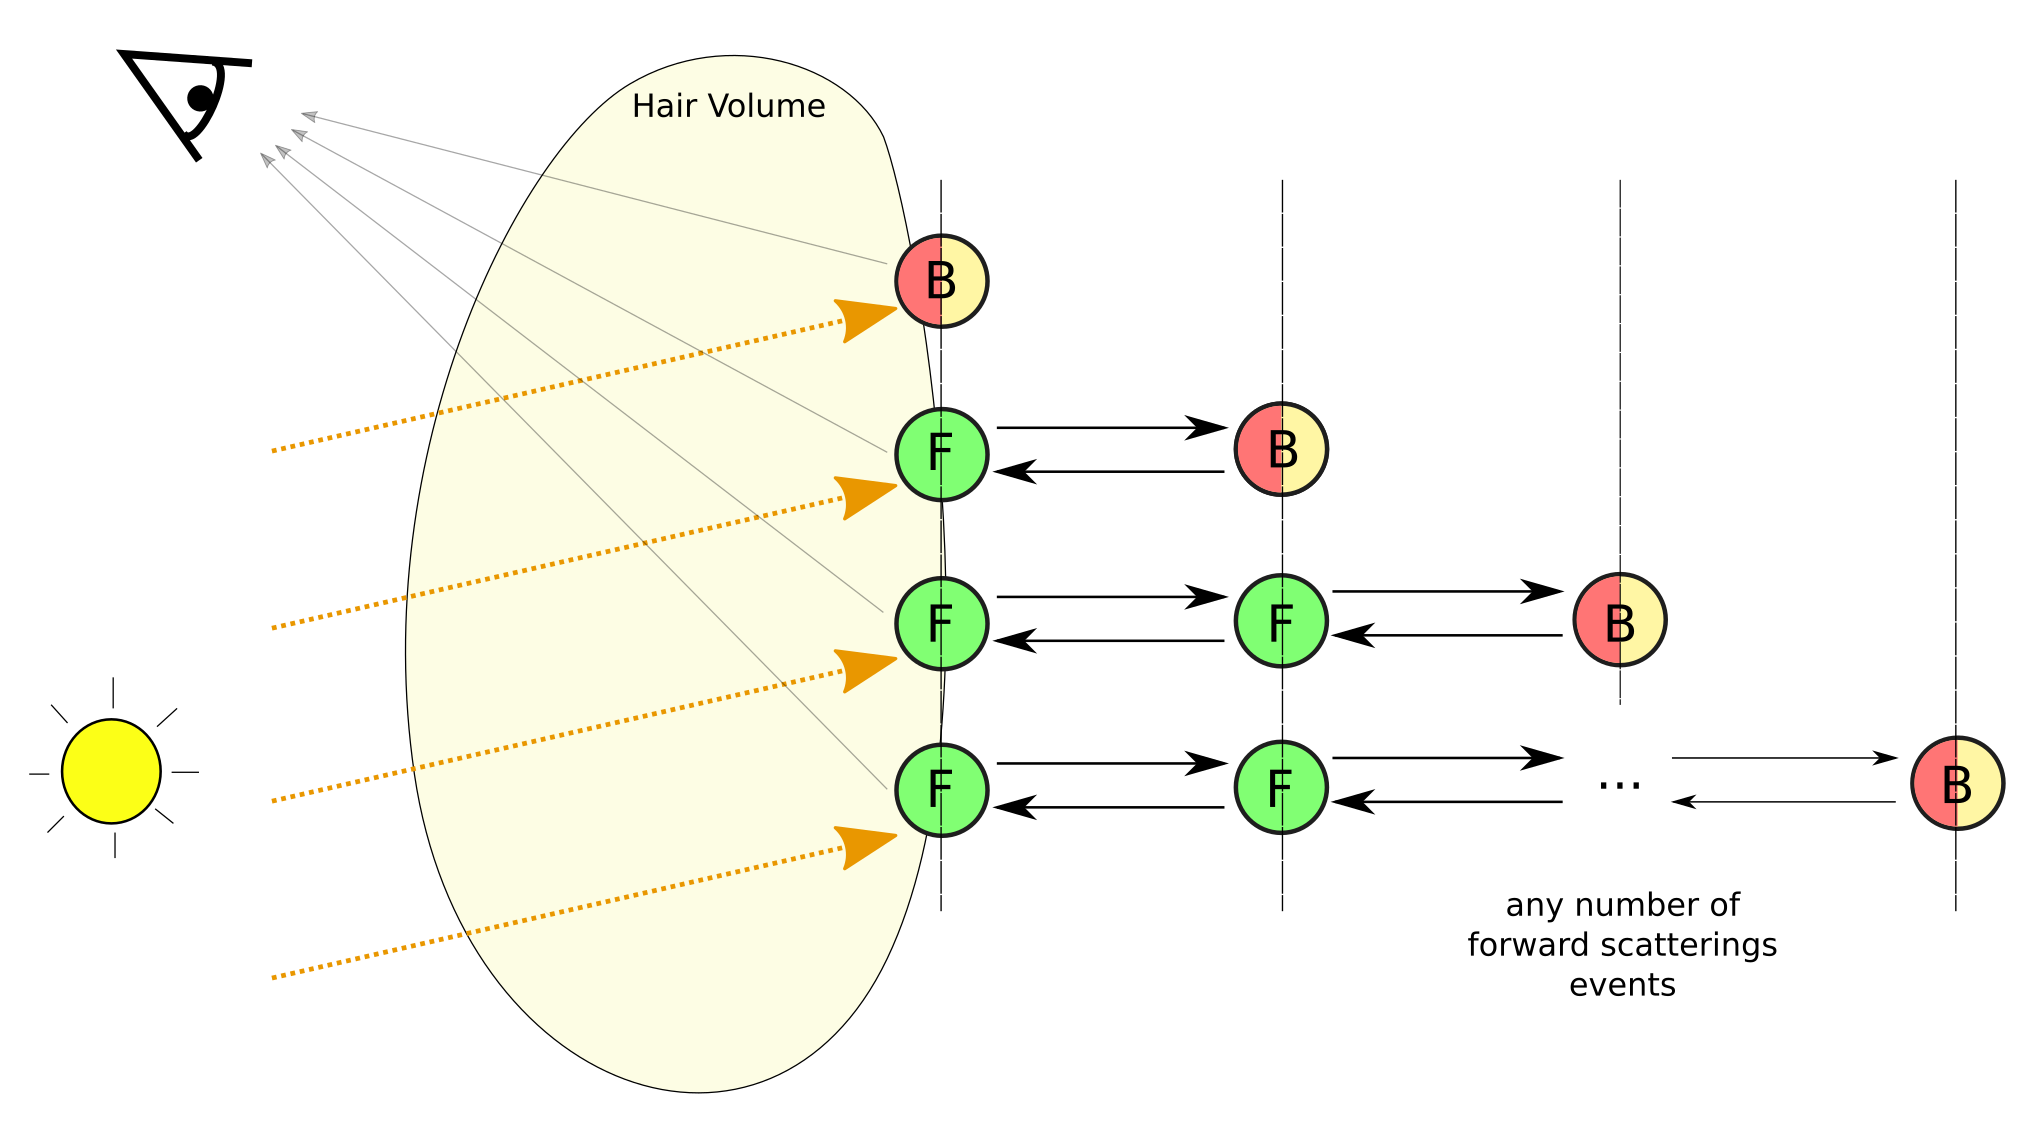
\includegraphics[scale=0.25]{avg_backscatter_1.png} \\
    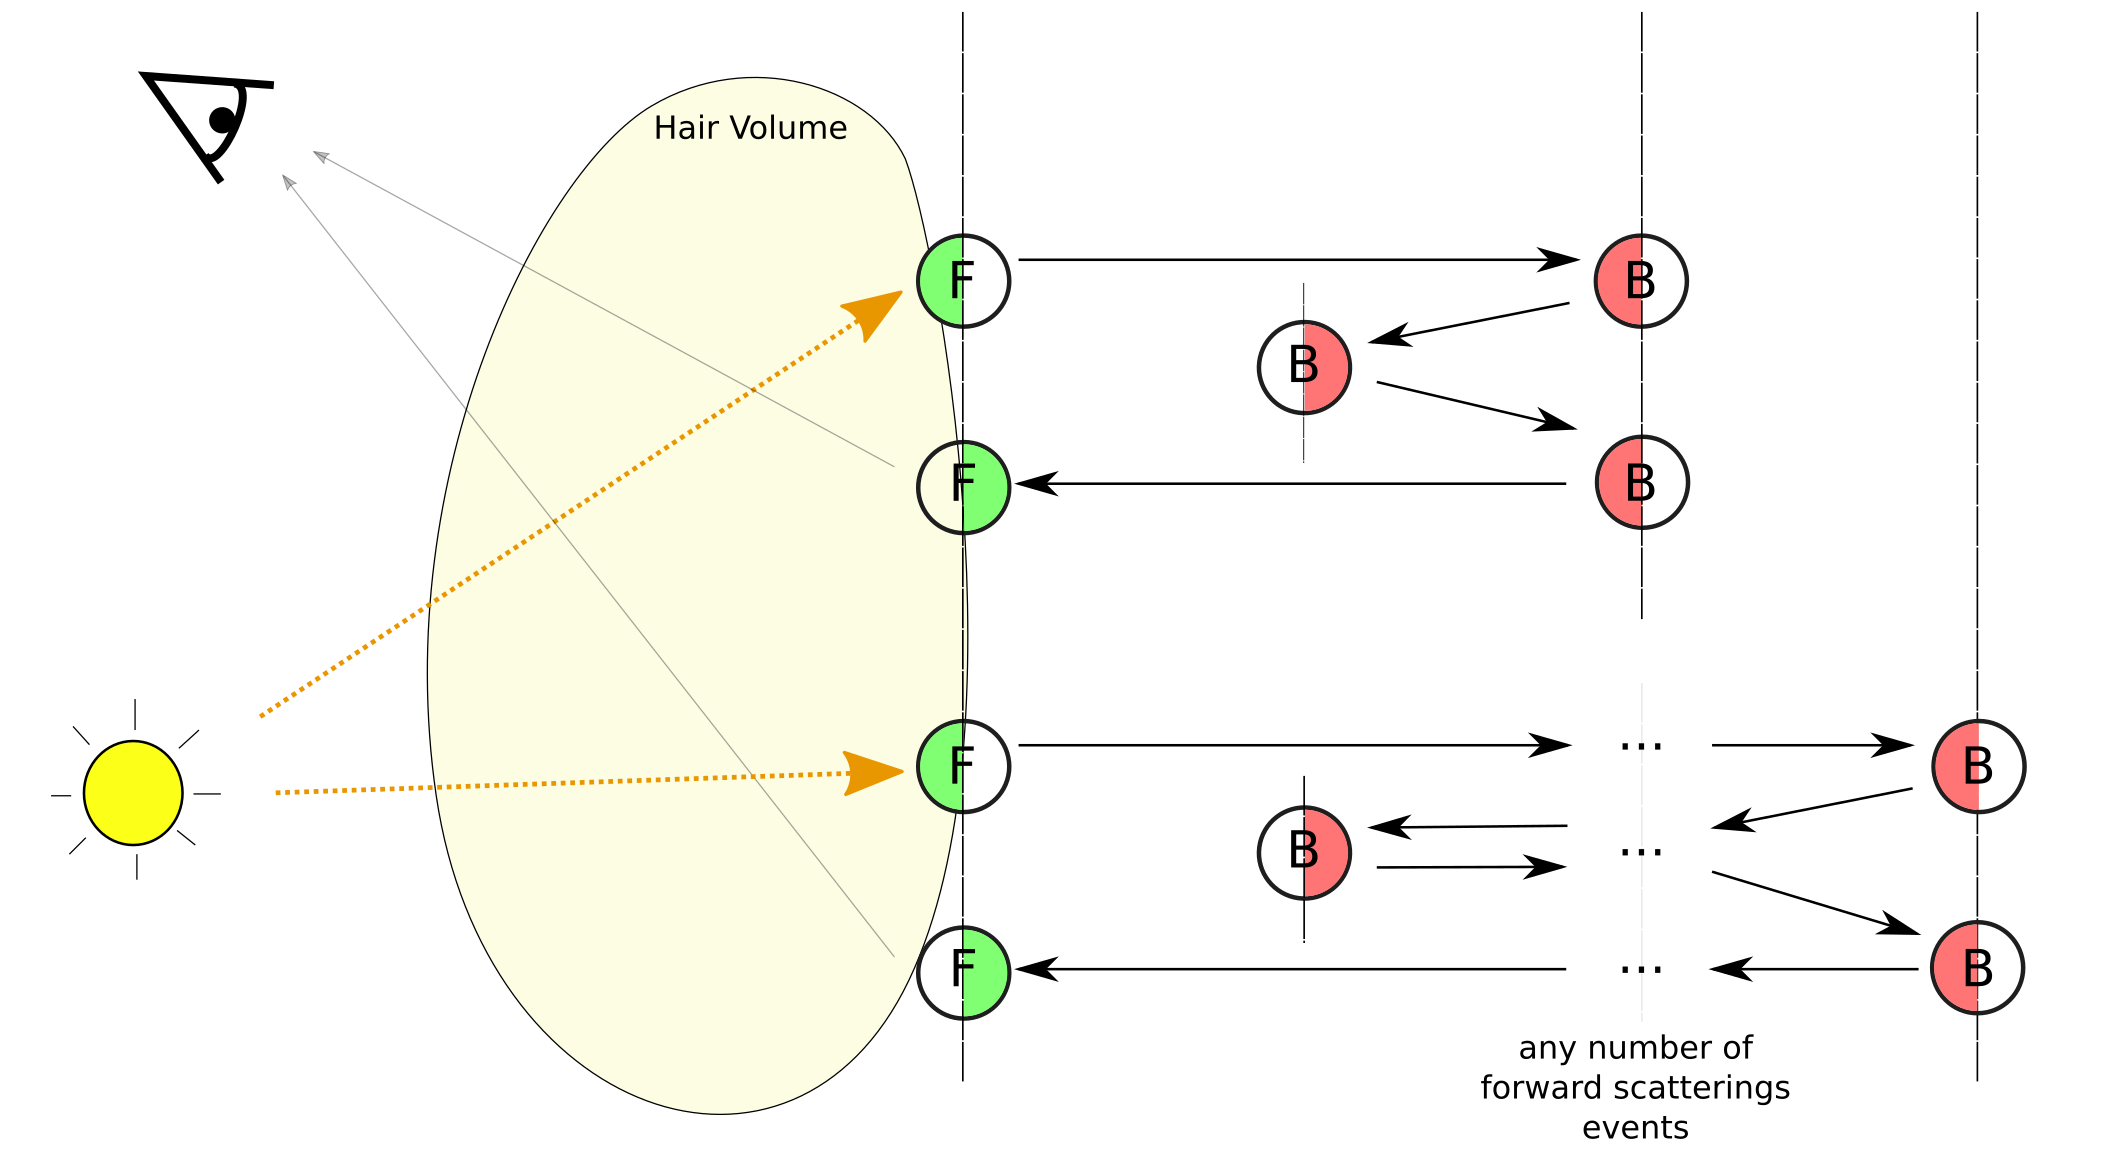
\includegraphics[scale=0.25]{avg_backscatter_3.png}
    \end{tabular}
    \caption{Visualization of the average backscattering attenuation $A_b$. The circles represent the cross section of the hair fibers. The color coded half circles represent the scattering event taking place, with red being a backward scattering event and green a forward scattering event, also indicated by B and F respectively. The orange ray correspond to the incident light from the light source. It represent the global illumination passing through the hair volume reaching the local neighborhood. The dual scattering method takes into account only one or three backscatter events. All permutations of one backscatter event ($A_1(\theta)$) is displayed in the top figure and all permutations for three backscatter events ($A_3(\theta)$) is displayed in the bottom figure. It is clear to see that the amount of
    forward scattering events may go to infinity, but that the amount of backscattering events is limited to one or three. This leads to the infinite series that can be written as shown in equation~\ref{avg_backscatter_series}.}
    \label{avg_backscatter_attenuation}
\end{figure}

\subsubsection{Average backscattering spread}

The average backscattering spread takes into account the loss of intensity, due to spreading of the light after backscattering events occur. This is similar to forward scattering events. The dual scattering method~\cite{zinke} presents the average backscattering spread $S_b(\omega_i, \omega_o)$ as

\begin{equation}
S_b(\omega_i, \omega_o) = \frac{s_b(\phi_i, \phi_o)}{\cos \theta} g(\theta_o + \theta_i - \Delta_b(\theta_d), \sigma_b^2(\theta_d)
\end{equation}

where $s_b$ equals $1/\pi$ for backward scattering directions and zero for forward scattering, $\Delta_b(\theta_d)$ is the average longitudinal shift caused by the scattering events.

The spread is modeled as a single gaussian function. It is important to notice that $\Delta_b$ represents the average mean and $\sigma^2$ represents the average variance, thereby taking into account the multitude of possible forward and backward scattering events.

The average longitudinal shift $\Delta_b$ and average longitudinal standard deviation $\sigma_b$ for backscattering can be precomputed by averaging over all directions. See the dual scattering method~\cite{zinke} for more details and ~\cite{sadeghi} for a more hands on approach.









\chapter{Approach}

The central problem in this thesis, and for rendering in general, is to reduce variance with the same amount of samples. Either by requiring less samples per pixel for the same quality image, or by increasing the quality of the image with the same amount of pixels. In both cases, it boils down to the same problem and this problem is usually solved by careful sample placement. Increasing the rendering speed is relevant for several applications, such as for the animation movie industry that wants to generate physically accurate movies, and for rendering real-time hair simulations for the cosmetic industry. In this thesis the choice is made to apply multiple importance sampling to the dual scattering method.

In this chapter the theoretical approach discusses the theoretical challenges involved in rendering hair models using importance sampling. Based on the literature provided in chapter ´Background', there is no official approach on how to apply importance sampling to the dual scattering method. This is where this chapter kicks in. In this chapter I will elaborate on how to importance sample the dual scattering method of Zinke et al.~\cite{zinke}.

The theoretical challenges are as follows:

\begin{itemize}
    \item[1] \textbf{How to apply multiple importance sampling to the dual scattering method?} 
    The multiple importance sampling algorithm that is applied to the dual scattering method has been created for the improved Marschner model. The challenge is that the dual scattering method forms a different basis to the importance sampling algorithm. It could work less optimal if the probability distribution for the importance sampling algorithm does not match accurately with the distribution of the dual scattering method. In section~\ref{approach_problem1} the design decisions are explained and in section~\ref{approach_problem3} the multiple importance scattering algorithm is explained in depth.
    \item[2] \textbf{How to measure or compare the results for multiple importance sampling?} Rendering images using multiple importance sampling can look nice, or more visually pleasing when more samples are taken, but it is important to be clear on how to evaluate rendered images. In section~\ref{approach_problem2} the evaluation criteria are expressed.
    \item[3] \textbf{The theoretical approach to implement multiple importance sampling in the PBRT framework.} Although PBRT is about the implementation of the algorithm, the framework requires an importance sampling function to be implemented in a specific way. This way has an impact on the theoretical approach.
\end{itemize}

In chapter~\ref{chapter_implementation} 'Implementation', the practical challenges are discussed that occurred when implementing a physics based hair rendering algorithm.



\section{Application of multiple importance scattering to the dual scattering method}
\label{approach_problem1}

Creating a multiple importance sampling strategy is a mathematically involved process. Except for the most simple mathematical distributions, it usually requires quite a lot of mathematical background theory in order to solve the complex integrals that follow from complex scattering distributions. This is one of the reasons why it is difficult to find an importance sampling strategy for the original Marschner model. This is also the reason why so much effort has been put in expressing the Marschner model using more simple mathematical equations. This is to make importance sampling possible as has eventually been accomplished by d'Eon et al.~\cite{eon2013}.

The current status in hair rendering can be summarized by the following two points.

\begin{itemize}
    \item The dual scattering method provides an approximation to rendering multiple scattered hair by breaking up the computations for single scattering and multiple scattering. Single scattering resembles the original Marschner model, but the more expensive multiple scattering has been replaced by a volume scattering approximation. It provides a speed up compared to the traditional Marschner model, where extensive path tracing is needed to compute the effects of multiple scattering through the hair volume.
    \item The original Marschner model has been extensively analyzed and improved. One of the improvements is that the expensive root-solving process is removed. Eventually d'Eon et al.~\cite{eon2013} improved the algorithm even further by proposing an importance sampling algorithm on top of the already improved Marschner model.
\end{itemize}

One of the observations made in d'Eon et al.~\cite{eon2013} is that the importance sampling strategy should work for the original Marschner model, as well as for all models that approximate the Marschner model. The observation behind this is that all approximated solutions to the Marschner model in essence are modeling the same scattering distribution. If the scattering distribution would be different, then the hair rendering would look different compared to the Marschner model. This means that the importance sampling should be able to be applied to the dual scattering method, since the dual scattering method approximates the Marschner model.

The only caveat is that the Marschner model is not fully energy conserving at the edge-cases, such as glancing angles. This problem is applicable to the dual scattering method as well. The expectation is that these edge-cases can be ignored and therefore the choice has been made that it is possible to apply the importance sampling strategy by d'Eon et al.~\cite{eon2013} to the dual scattering method of Zinke et al.~\cite{zinke}. The details on the multiple importance sampling strategy are elaborated in section~\ref{approach_problem3}.





\section{Evaluation of rendered images generated by multiple importance sampling}
\label{approach_problem2}

The main goal of this thesis is to find out if multiple importance sampling applied to the dual scattering method leads to a significant reduction of noise in the rendered image. In order to come to a conclusion, evaluation criteria need to be set up. This is a challenge since there is no reference image to compare with. There are three criteria to take into account:

\begin{itemize}
    \item Which sampling technique to use to render the reference material?
    \item How many samples per pixel to use for comparing rendered results?
    \item How to evaluate the reference image with the multiple scattered image?
\end{itemize}

The reference image will from now on be named the ground truth. In this thesis the ground truth image is rendered using the same dual scattering implementation as the multiple importance sampled results. The difference is only in the way of sampling, where the ground truth is rendered using uniform sampling. Uniform sampling can be considered a typical way of sampling when the distribution is unknown, and therefore a valid way to compare the multiple importance sampled results with. By changing only the sampling strategy, the resulting noise can be compared pixel by pixel. 

The idea behind unbiased sampling strategies is that they all converge to the same result. Using this property, the expectation is that by taking a lot of samples, the result of uniform sampling and importance sampling should be equivalent. For this thesis, the ground truth is rendered up to 512 pixels per sample. This does not completely remove the noise from the ground truth, but it is sufficient to perform a comparison. Especially with importance sampling, you should see the impact clearly for a low amount of samples. Also, taking more samples drastically increased rendering times. 

At last an evaluation needs to be performed. In this thesis, the rendered results are compared for an incremental number of samples per pixel, from 1 up to 512 samples per pixel. To evaluate whether importance sampling reduces noise, two comparisons are performed.

\begin{itemize}
    \item First of all a comparison is made by comparing the visual appearance of the image. Is the result obtained with importance sampling looking as we expect for different scenarios? Such as when the model is backlit or frontlit, or when the amount of reflection is high? This comparison is rather subjective, so there needs to be another unbiased way to measure the performance between uniform and importance sampling.
    \item Second, a comparison is performed between the variance in the rendered result. It is important to only compute the variance for the hair volume and not for the background image. This could otherwise give us a false sense of conversion if the hair model covers only a small region of the image. To prevent this from happening, only a specific rectangular region of the image is taken into account that is fully covered by the hair model. The variance is then only computed for this specific region. Figure~\ref{fig_variance_outline} visualizes the comparison region.
\end{itemize}


\section{Theoretical approach to multiple importance sampling for the dual scattering method}
\label{approach_problem3}

As mentioned a couple of times before in this report, d'Eon et al.~\cite{eon2013} proposed a physically based importance strategy for the improved Marschner model (also by d'Eon et al.~\cite{eon2011}). This strategy should work for the original Marschner model as well. In this section the theoretical details of this physically based importance sampling strategy is explained and how it is applied to the dual scattering method. 

As has been explained in section~\ref{section_importance_sampling} faster convergence can be obtained by using importance sampling over uniform sampling. The challenge with importance sampling is to sample an incoming light direction $\omega_i$, given an outgoing direction $\omega_o$. This is how it works in PBRT and most physics based system. The outgoing direction could be treated as the direction to the viewer or camera (at least for the first ray). The challenge is two fold: find a sampling distribution that matches the scattering behavior, and subsequently find an efficient way to sample the scattering distribution. If you are lucky, the scattering distribution is not complex and a sampling algorithm is trivial to find. If the distribution is too specific or complex, it might actually be impossible to analytically come to a sampling strategy.

The reason why the theoretical details are explained in the approach chapter is that the translation from the algorithm to code is rather challenging. The challenge comes from the way what PBRT expects an importance sampling algorithm to be provided. In general there are two situations that need to be handled when implementing an importance sampling strategy in PBRT.

\begin{itemize}
    \item Sampling an incident (light) direction $\omega_i$, given an outgoing (viewing) direction $\omega_o$. The used probability distribution function should ideally be a close fit to the scattering distribution of the hair rendering model. Also the corresponding PDF should be computed, which is the likelihood of the sample being drawn.

    \item Compute the PDF for two given directions $\omega_i$ and $\omega_o$, This is similar to the previous point, except that the output is now only a PDF value.
\end{itemize}

The scattering function for the Marschner model is given in equation~\ref{marschner_model_scatterfunction}. D'Eon et al.~\cite{eon2011} simplified this equation so that the longitudinal scattering function $M$ is only dependent on longitudinal angles, and the azimuthal scattering function $N$ is only dependent on the azimuthal angles. Also the inclination dependent factors, such as the $\cos^2 \theta_d$ term, present in the original Marschner model are included in the $M_p$ term. This leads to the following simplified equation:

\begin{equation}
    \label{eq_model_S}
    S_p(\omega_i, \omega_r) = M_p(\theta_i, \theta_o) N_p(\theta_i, \theta_o, \phi)
\end{equation}

\subsection{Strategy outline}

In this section the multiple importance sampling strategy for the Marschner model is explained. The strategy comes from d'Eon et al.~\cite{eon2013} and is summarized here.

The idea behind the importance sampling strategy is to seperate the sampling for the longitudinal scattering function and for the azimuthal scattering function, hence we do have multiple importance sampling. Multiple importance sampling is nothing more than a combination of two or more importance sampling strategies combined into a single \"multiple\" importance strategy.

The basic outline of the strategy is as follows.

\begin{itemize}
\item Select a lobe $p \in \{ \textnormal{R}, \textnormal{TT}, \textnormal{TRT} \}$ dependent on the relative contribution of energy reflected. This depends on the Fresnel equation and the absorption coefficient $\sigma$.
\item Given a selected lobe $p$, compute the longitudinal angle by sampling the longitudinal scattering function $M_p$.
\item An outgoing direction $\omega_o$ is given, so we know the spherical angles $\theta_o$ and $\phi_o$.
\item Choose a random offset $h \in [-1, 1]$ along the fiber cross section.
\end{itemize}

The following subsections delve deeper into the items mentioned above.

\subsection{Lobe selection}
\label{sec_lobe_selection}

When importance sampling incident directions, we want to take into account the relative contribution of the different lobes in the model. For example, the R component has a stronger influence when viewing hairs from glancing angles compared to the other reflection modes. In that case you want to prefer sampling an incident direction based on the reflection component. Likewise, hair strands that are backlit do have more contribution from the TT component. It is important to take this into account, because for importance sampling we prefer to sample directions that have more impact (or weight) on the rendered result than just random sampling. With random sampling a lot of samples could be wasted, for example by taking into account the TRT component when the R reflection is much more dominant in the rendered result.

d'Eon et al.~\cite{eon2013} proposes a way to select lobes by taking into account the attenuations through a smooth, ideally specular fiber $A_{\textnormal{spec}}(p, h)$. The strategy is to first select a random cross-section offset $h = 2\xi_h - 1$,  where $\xi_h \in [0, 1)$ is a uniformly distributed random number. Once the random cross-section offset is known, we can compute the relative contributions for each of the scattering modes. The relative contributions for the scattering modes are as follows, where 0 corresonds to R, 1 corresponds to TT and 2 corresponds to the TRT scattering mode.

\begin{align}
A_{\textnormal{spec}}(0, h) &= F(\eta, \gamma_i) \\
A_{\textnormal{spec}}(1, h) &= (1 - F(\eta, \gamma_i))^2 \, T(\sigma_a, h) \\
A_{\textnormal{spec}}(2, h) &= (1 - F(\eta, \gamma_i))^2 \, F(\frac{1}{\eta}, \gamma_t) \, T(\sigma_a, h)^2
\end{align}

These values describe the relative amount of energy transmitted through or reflected against hair fibers for each of the scattering modes. We do not yet take into account rough fibers, so all energy is concentrated in the specular direction. To sample a lobe these contributions should be related to the sum of all contributions to find the relative weights $w_p$.

\begin{align}
w_{\textnormal{R}} &= \frac{A_{\textnormal{spec}}(0, \gamma_i)}{\sum_p A_{\textnormal{spec}}(p, \gamma_i)} \\
w_{\textnormal{TT}} &= \frac{A_{\textnormal{spec}}(1, \gamma_i)}{\sum_p A_{\textnormal{spec}}(p, \gamma_i)} \\
w_{\textnormal{TRT}} &= \frac{A_{\textnormal{spec}}(2, \gamma_i)}{\sum_p A_{\textnormal{spec}}(p, \gamma_i)}
\end{align}

Given the relative weights, a lobe can be sampled by taking a random uniform variable $h \in [0, 1)$ and selecting a lobe proportional to the relative attenuation of each component. Once the lobe is selected, importance sampling the longitudinal and azimuthal scattering functions becomes relatively straightforward.

The PDF of the sampling scheme is exactly analogous to evaluation of the model $S$ in equation~\ref{eq_model_S}, but with the attenuations $A$ replaced by the selection weights $w_p$. By replacing the attenuations with the sample weights, the PDF is always integrating to 1 irrespective of the hair color.


\subsubsection{Finding the PDF when directions $\omega_o$ and $\omega_i$ are known}

The PBRT framework requires a function to compute the PDF given two directions $\omega_o$ and $\omega_i$. As stated in the previous section the PDF is analogous to the evaluation of the model $S$, but with the attenuations replaced by the selection weights $w_p$. The selection weights were determined before by sampling a cross section, giving us the relative contribution per scattering component and thus eventually the relative direction to be sampled.

When $\omega_o$ and $\omega_i$ are known, the PDF cannot be found by sampling from a cross section. In this case, the relative direction between the angles is used. All scattering modes could produce the difference angle, although for some scattering modes it would be more likely. In this case the process is inverse and instead of selecting a lobe given the outgoing direction, now we should take into account the likelihood of each scattering component sampling the given incident direction.

This is done by solving for roots as has been explained in the related work section~\ref{sec_marschner}. The R and TT components have exactly one root and the TRT component results in one or three roots. This means that any scattering mode could have been selected that would result in the incident direction being sampled. In other words, we need to know the relative probability of a root $h$ to be selected for each of the R, TT and TRT scattering modes, given $\omega_i$ as a sampled direction.

This is done in a similar way to sampling a lobe by using the relative attenuation for each of the roots $h$. Since the TRT component can have three roots, it means that this scattering mode actually has three paths to generate the sampled direction. They are summed together to represent the attenuation for the TRT mode. The relative attenuations are then used as the sample weights when evaluating the model $S$ to find the corresponding PDF.

\subsection{Importance sampling the longitudinal M function}
\label{sec_importance_sampling_M}

To importance sample the longitudinal scattering function $M$, we need a way to sample a gaussian distribution. The essence here is that we are given the outgoing direction $\omega_o = (\theta_o, \phi_o)$ and we need to find the incident longitudinal angle $\theta_i$. The incident $\phi_i$ is determined in the next section (when importance sampling the azimuthal scattering function $N$).

There is a problem with the gaussian distribution of the Marschner model. First of all it is not energy conserving as has been explained before in section~\ref{marschner_longitudinal_scattering_function}. Part of this can be solved by multiplying the half angle $\theta_h$ by two. Another problem is that especially at glancing angles, part of the energy falls outside of the boundary $\theta \in \{ -\pi/2, \pi/2 \}$, thereby losing energy. This is a problem for importance sampling. When energy is outside of the allowed range, we must somehow compensate this loss of energy in the remaining part of the gaussian distribution. This is pretty difficult to achieve, at least with the simple normalized gaussian distribution ranging from $\theta \in \{ -\infty, \infty \}$.

d'Eon et al.~\cite{eon2011} proposes a different energy-conserving longitudinal scattering function $M_p$. This function conservatively redistributes reflected radiance amongst directions on the sphere by employing spherical gaussian convolution. This function is energy conserving and makes sampling a lot easier. The newly used energy conserving scattering function $M$ is as follows:

\begin{equation}
M_p(v, \theta_i, \theta_r) = \frac{\textnormal{csch}(1/v)}{2v} e^{\frac{\sin(-\theta_i)\sin\theta_r}{v}} I_0 \Big [ \frac{\cos(-\theta_i) \cos \theta_r}{v} \Big ]
\end{equation}

where $v$ is the longitudinal scattering variance ($\beta_p^2$) and $I_0$ is the modified Bessel function of the first kind. In the implementation, the Bessel function is available in the Boost library. Another option is to use the Python scientific programming library (scipy) and store the results in a lookup table.

Using the conserving scattering function, instead of the original Marschner scattering function is not an issue. This is the power of importance sampling, to be able to sample an arbitrary complex function (the marschner model) using a simpler and easier to sample function (the conserving scattering function). As long as the function is a good fit, variance will be reduced. More information about the derivation of this function and why it works can be found in the paper by d'Eon et al.~\cite{eon2011}.\\

Sampling a spherical gaussian can be done with two random numbers $\xi_1$ and $\xi_2$ each within $[0, 1)$. Using the Box-Muller transform gives us a sample for the normalized spherical gaussian function. The computation requires a lot of mathematics, which is explained in the paper by d'Eon et al~\cite{eon2013}. The strategy to find the sampled $\theta_i$ is as follows.

\begin{align}
u(\xi_1) &= v \log \Big (e^{1/v} - 2\xi_1 \sinh \frac{1}{v} \Big ) \\
\theta_{\textnormal{cone}, p} &= -\theta_i + \alpha_p\\
\theta' &= \frac{\pi}{2} - \theta_{\textnormal{cone}} \\
\theta_i(\xi_1, \xi_2, v, \theta_{\textnormal{cone}}) &= \nonumber \\
& \arcsin(u(\xi_1) \cos \theta' + \sqrt{1 - u(\xi_1)^2} \cos(2\pi \xi_2) \sin \theta')
\end{align}

The probability of sampling this value is equal to the longitudinal scattering function $M$, assuming that the scattering distribution is energy conserving and integrates to 1, so the the PDF is $M \cos^2 \theta_i$.

\subsection{Importance sampling the azimuthal N function}

Importance sampling the azimuthal $N$ function is trivial if we know the selected lobe $p$ and the offset $h$ from the scattering cross section (see section~\ref{sec_lobe_selection}). In that case it is a matter of evaluating the relative change in azimuth $\Phi(p, h)$ (see equation~\ref{eq_relative_azimuth_change}). To find the incident azimuth direction $\phi_i$.

\begin{align}
\label{phi_func}
\phi_i^{\textnormal{smooth}} &= \phi_o + \Phi(p, h)
\end{align}

For rough fibers, the relative change in azimuth is offset by a gaussian distributed random variable $g$ with standard deviation 1, multiplied by the width $\beta_p$ corresponding to the selected lobe $p$. Sampling a gaussian distribution can be performed using the Box-Muller transform as explained in the previous subsection. The direction $\phi_i$ to be importance sampled can then be found as follows:

\begin{align}
\phi_i &= \phi_o + \Phi(p, h) + g | \beta_p | 
\end{align}

Take into account that the spherical direction wraps around in the range $\{ -\pi, \pi \}$.


\chapter{Implementation}
\label{chapter_implementation}

Aside from the theoretical challenges, there are also practical challenges in implementing physics based rendering algorithms, especially when dealing with hair models that often consist of hundreds of thousands of hair fibers. These hair fibers which are huge in amount, are also very thin, especially compared to the projected area on a pixels.

This chapter deals with the implementation details to implement the importance sampling strategy for the dual scattering method. The theoretical approach is described in the previous chapter. The practical challenges can be summarized as follows.

\begin{itemize}
    \item[1] The choice of the framework to render physics based algorithms in combination with the representation of hair strands (section~\ref{sec_which_framework}).
    \item[2] Representation of the voxel grid (section~\ref{sec_voxel_grid}).
    \item[3] Dealing with memory and speed requirements (section~\ref{sec_memory_requirements}).
    \item[4] The non-intuitiveness of the Marschner model parameters (section~\ref{sec_nonintuitiveness_marschner}).
\end{itemize}

The next sections will address these challenges on how these are tackled in this thesis.


\section{The choice of the physics based rendering framework}
\label{sec_which_framework}

The first challenge is to find a proper ray tracing framework, which offers the possibility to write your own BSDF materials. There is a lot of choice between different renderers, but one that is extremely useful is PBRT. PBRT stands for Physics Based Ray Tracing and is used a lot to explore and experiment with physics based raytracing algorithms. It is developed by Matt Phar et al. and freely available, open source from their website~\footnotetext{http://www.pbrt.org} and described in their corresponding book~\cite{pbrt}. The rendered images in this thesis are created using PBRT.

Within PBRT, it is possible to create your own BSDF's. A BSDF is usually applied to a surface as has been discussed in section~\ref{sec_bsdf}, but for hair rendering we are using curve representations. The curve variant of a BSDF is called a "bidirectional curve scattering distribution function", abbreviated as BCSDF. PBRT provides a generic solution using BxDF classes in which it is possible to represent BCSDF materials.

The representation of hair fibers can be done in a variety of ways as has been discussed in section~\ref{sec_geometric_complexity}. The possibilities were to represent them as connected triangle strips, cylindrical primitives, trigonal prisms or ribbons. Within PBRT hair fibers are specified as curves, which are a sequence of cubic Bezier splines represented by 3D points. For every cubic spline segment, the width is specified. PBRT has support for three types of curves: flat, cylindrical or ribbons. Flat corresponds to triangle strips, and the other curve types are self-explanatory. For the rendered results in this thesis cylindrical curves are used, which correspond to the most realistic representation.

\section{Representation of the voxel grid}
\label{sec_voxel_grid}

Voxel grid implementations are not that trivial as they might seem at first. Yes, you can use a three-dimensional array, but this is not efficient for rendering purposes. One of the problems with voxel grids are the hard edges they produce in the renderings. Making the voxel cells very small leads to memory issues, or even precision issues because of their small size.

The dual scattering approximation requires a way to efficiently approximate the global multiple scattering. The global multiple scattering can be computed in a number of ways. Zinke et al.~\cite{zinke} proposed the following methods:

\begin{itemize}
    \item Ray-shooting: with ray-shooting a shadow ray is shot through the hair volume, calculating the number of intersections with the hair fibers, together with the angle the ray makes with the direction of the fiber. In this way the density can be approximated using the formulas as explained in the background theory on dual scattering ~\ref{sec_dualscattering}. This strategy is the simplest but most expensive one to compute, because of the number of intersections being computed. Also this strategy is a little tedious to implement in PBRT. The reason for this, is that PBRT is build on the fact that every intersection is a material intersection. Tracing a shadow ray through a volume, just to count the number of intersections, is actually something non-physical and therefore not supported out of the box.
    \item Forward-scattering maps: with forward scattering maps a two-pass approach is made. First a voxel grid is precomputed in which every voxel cell contains containing the average values for the forward transmittance $T_f$ and forward longitudinal spread $\sigma^2_f$. During the second pass, linear interpolation is used to integrate along the ray through the voxel grid.
    \item GPU rendering using deep-opacity maps: this solution is very fast, but contains some tricks using deep opacity maps and a preprocessing step where depth maps are calculated. This thesis primarily focuses on physics based approaches and therefore didn't went in this direction.
\end{itemize}

The most plausible approach for this thesis is the second option: a two pass approach in which a voxel grid is precomputed. From the explanation it follows that the voxel grid should contain a possibility to do linear interpolation along a path. Also from a practical perspective, the voxel grid should not consume too much memory. For this thesis, an open-source software package OpenVdb is used~\footnote{http://www.openvdb.org}. OpenVDB is developed at Dreamworks Animation and is especially suited to be used when rendering volumetric effects. It is able to store sparse voxel grids without consuming much memory and with support for different ways of sampling: point, box and quadratic sampling that correspond to averaging out the sample based on the value in the neighboring voxel cells.

In this thesis the preprocessing step works as follows. For every hair fiber that is represented as a curve, loop through the curve by a specific offset, and for each position, find the corresponding voxel cell. This voxel cell is incremented with the length of the curve segment. In this way, all voxel cells, contain the relative lengths that have been traversed in that voxel cell. These lengths do not necessarily correspond to absolute density values, but are relative density values. When rendering a hair model, the density can be scaled to adjust the rendered result. In this thesis I decided not to store the orientations per voxel cell. This is a simplification. The reason I chose for this simplification is that hair fibers are usually similar in orientation in their local neighbourhood. Also it makes the voxel generation process less complex. For more realistic behavior that is applicable to more complex hair models, the orientations of the fibers should be taken into account.

In the second pass the hair model is rendered. If the ray intersects with the first hair fiber at the surface of the hair volume, a lookup is performed in the voxel grid. The voxel grid, based on 3D location and orientation, is used to traverse through all voxel cells along this \"shadow\" ray, integrating the results using box sampling. The choice for box sampling is arbitrarily, because the results were nice enough. It could be worth to do further research on choosing different sampling algorithms and on determining the best possible voxel size for different types of hair models such as straight hair versus curvy hair.

One experienced side effect of integrating the density through the voxel grid, is for intersections at the hair volume boundary. The first fiber hit is not in shadow. This is evident, since it's located at the boundary edge. However, looking up the density value gives an indication that the fiber is in shadow. This is solved by tracing an additional shadow ray to the light source to decide whether it has a clear path to the light source. If that is the case, no lookup is performed and it is assumed the hair fiber is fully lit without strands covering it.

\section{Dealing with memory and speed requirements}
\label{sec_memory_requirements}

Rendering hair models is very slow. The system configuration that I used for rendering is a quad core Intel Core i7-3770K processor with 8 gigabytes of RAM. Rendering times for 512 samples per pixel would lead to a couple of hours. The curvy hair model was not possible to render at all, because it consumed more memory than the 8 GB of available RAM. The system therefore resorted to virtual memory, practically stalling the rendering process. The reason why memory usage is so high, is because bookkeeping structures are needed by PBRT to improve ray intersections.

One of the tricks that is performed in this thesis is to render only half of the hair model, where the 'removed' half of the hair model is pointing away from the camera. In this way, it is not visible that actually half the hair model is used during rendering. The voxel generation process is still using the full hair model to reflect that the density is still there, even though half the hair volume is actually removed. Another way to speed up the rendering during debug times is to render only a subframe of the image, so that quick feedback loops are possible after only half a minute of rendering.

\section{The non-intuitiveness of the Marschner model parameters}
\label{sec_nonintuitiveness_marschner}

The Marschner model is a physically based hair rendering model. It is based on physical properties, such as the absorption of light propagating through the core of the hair fibers, the curvature of the hair cylinder, the width and shift of the scattering lobes and many more. These parameters are non-intuitive from the perspective of an artist wanting to achieve the perfect look. They are also non-intuitive for me to be able to render distinct effects of the Marschner model, such as the TRT component which is hard to visualize clearly. This was a challenge when creating rendered results.


\chapter{Results}

In this chapter results are presented. First the dual scattering model is presented in a variety of settings. Then the effect of the average forward and backward density factors are shown, followed by a numerical analysis by using variance to compare the noise between uniform sampling and importance sampling.

This thesis is very mathematically involved with a lot of background knowledge required in both mathematics and physics. One of the contributions of this report is therefore my personal knowledge gain in these fields.


\section{Dual scattering in real-world situations}

Usually when rendering, multiple importance sampling is performed to take samples from the light source and samples determined by the material. If the light source would be small, then taking samples determined by the light source will usually always give better results then using importance sampling from the material. To be able to see the effect of importance sampling for the hair material, we thus must make sure that we have a globally illuminated scene, to see the difference between importance sampling and uniform sampling.

The results presented in this section compares results from uniform sampling with results from importance sampling. The models are placed in a global illuminated scene, where global illumination is accomplished by using HDR spherical environment maps.

In figure~\ref{fig_officesquare},~\ref{fig_venice} and~\ref{fig_subway} results are presented for different real world scenarios. The images are presented to give a realistic impression on how the dual scattering method performs between uniform and importance sampling for 32 samples per pixel. The scenarios are presented in full daylight with the sun shining on the hair model, in a daylight setting where there is no direct impact of sunlight and an indoor setting in a subway station that lacks a lot of light. Especially in daylight scenerios it is clear that the color of the hair model is apparent. In darker situations, only the blond hair distinguishes itself from the colored hair types. This is expected, because colored hair types absorb much more light than blonde hair.


\begin{figure}[H]
\centering
\begin{tabular}{cc}
Uniform Sampling (32 samples) & Importance Sampling (32 samples) \\
\includegraphics[scale=0.16]{realworld/officesquare/uniform_blonde1_32.png} & \includegraphics[scale=0.16]{realworld/officesquare/deon_blonde1_32.png} \\
\includegraphics[scale=0.16]{realworld/officesquare/uniform_black1_32.png} & \includegraphics[scale=0.16]{realworld/officesquare/deon_black1_32.png} \\
\includegraphics[scale=0.16]{realworld/officesquare/uniform_brown2_32.png} & \includegraphics[scale=0.16]{realworld/officesquare/deon_brown2_32.png} \\

\end{tabular}
\caption{Comparison between importance sampling and uniform sampling in an office square setting. There is a lot of daylight, but no direct sunlight on the hair models. The reflection of the glass windows is clearly visible in the hair volumes. The images are rendered using 32 samples per pixel.}
\label{fig_officesquare}
\end{figure}

%
% Venice square
%

\begin{figure}[H]
\centering
\begin{tabular}{cc}
Uniform Sampling (32 samples) & Importance Sampling (32 samples) \\
\includegraphics[scale=0.16]{realworld/venice/uniform_blonde1_32.png} & \includegraphics[scale=0.16]{realworld/venice/deon_blonde1_32.png} \\
\includegraphics[scale=0.16]{realworld/venice/uniform_black1_32.png} & \includegraphics[scale=0.16]{realworld/venice/deon_black1_32.png}\\
\includegraphics[scale=0.16]{realworld/venice/uniform_brown2_32.png} & \includegraphics[scale=0.16]{realworld/venice/deon_brown2_32.png} \\

\end{tabular}
\caption{Comparison between importance sampling and uniform sampling in a bright daylight setting. The samples are rendered using 32 samples per pixel.}
\label{fig_venice}
\end{figure}

%
% Interior dark setting
%

\begin{figure}[H]
\centering
\begin{tabular}{cc}
Uniform Sampling (32 samples) & Importance Sampling (32 samples) \\
\includegraphics[scale=0.16]{realworld/subway/uniform_blonde1_32.png} & \includegraphics[scale=0.16]{realworld/subway/deon_blonde1_32.png} \\
\includegraphics[scale=0.16]{realworld/subway/uniform_black1_32.png} & \includegraphics[scale=0.16]{realworld/subway/deon_black1_32.png} \\
\includegraphics[scale=0.16]{realworld/subway/uniform_brown2_32.png} & \includegraphics[scale=0.16]{realworld/subway/deon_brown2_32.png} \\

\end{tabular}
\caption{Comparison between importance sampling and uniform sampling in a dark subway setting. This is a subway station platform, where the lights in the station are the direct lighting, and reflections from the walls and floor the indirect lighting. Since the absorption in blonde hair is relatively low, this model clearly stands out compared to the colored hair models that appear very dark. The images are rendered using 32 samples per pixel.}
\label{fig_subway}
\end{figure}

\subsubsection{Observations}

By observing the results uniform sampling seems to appear a bit more noisy, but not in such amount that you could call it a significant difference. Also it shows that the blonde hair model is the brightest of all. Especially in the subway setting (figure~\ref{fig_subway}) the blond hair still resembles blond hair, while the other two hair models are very dark. You can hardly see a distinction between black and brown hair.
Black hair in general has a minimal amount of global multiple scattering, because the absorption coefficient is so high. Light passes through this hair in minimal amount, therefore appearing black. The only effect visible in black hair is a direct reflection according to the reflection (R) component.


\section{Variation of the forward and backward density factors}

Figure~\ref{fig_results_df} shows the effect of changing average forward and backward density values $d_f$ and $d_b$. When the density factors are zero, the appearance boils down to single scattering. This is because a density factor of zero indicates that no global multiple scattered light reaches the shading points (refer to figure~\ref{fig_df} for a visual representation).

% +----
% Results varying df-db
% +-----


\begin{figure}[H]
\bgroup
\setlength{\tabcolsep}{0.0em} % for the horizontal padding
\def\arraystretch{0.0}%  1 is the default, change whatever you need
\begin{tabular}{cccc}
0.00 & \includegraphics[scale=0.12]{dbdf-results/brown_dbdf_0_00.png} & \includegraphics[scale=0.12]{dbdf-results/blonde_dbdf_0_00.png} & \includegraphics[scale=0.12]{dbdf-results/black_dbdf_0_00.png} \\
0.25 & \includegraphics[scale=0.12]{dbdf-results/brown_dbdf_0_25.png} & \includegraphics[scale=0.12]{dbdf-results/blonde_dbdf_0_25.png} & \includegraphics[scale=0.12]{dbdf-results/black_dbdf_0_25.png} \\
0.50 & \includegraphics[scale=0.12]{dbdf-results/brown_dbdf_0_50.png} & \includegraphics[scale=0.12]{dbdf-results/blonde_dbdf_0_50.png} & \includegraphics[scale=0.12]{dbdf-results/black_dbdf_0_50.png} \\
0.75 & \includegraphics[scale=0.12]{dbdf-results/brown_dbdf_0_75.png} & \includegraphics[scale=0.12]{dbdf-results/blonde_dbdf_0_75.png} & \includegraphics[scale=0.12]{dbdf-results/black_dbdf_0_75.png} \\
1.00 & \includegraphics[scale=0.12]{dbdf-results/brown_dbdf_1_00.png} & \includegraphics[scale=0.12]{dbdf-results/blonde_dbdf_1_00.png} & \includegraphics[scale=0.12]{dbdf-results/black_dbdf_1_00.png} \\
\end{tabular}
\egroup
\caption{A variation of the density factors $d_f$ and $d_b$, corresponding to the amount of global multiple scattering in the hair model. A value of 0 indicates the absence of global multiple scattering and 1 the full presence of global multiple scattering. Usually the value is set to a constant value 0.7.}
\label{fig_results_df}
\end{figure}

The results show that the global multiple scattering component is very important to the appearance of blond hair models. To a lesser extend, but still important, to brown hair models. For black hair models the global multiple scattering is hardly visible. This is in accordance to what is expected, because light colored hair types have by definition less attenuation when light propagates through hair fibers. Therefore there is more global multiple scattering through the hair volume.

\section{Theoretical Results}

In this section theoretical results are obtained based on measured data. As discussed in the approach the variance is used to quantify the errror compared with the ground truth. By varying the samples per pixel an insight is gathered in the convergence rate and the efficiency of the importance sampling strategy compared with uniform sampling. Figure~\ref{fig_variance_outline} displays a rendering of a curly brunette with an outline indicating the region of interest for variance computation. In subsequent sections, this region is used for variance computation. This is done so that the background image has no effect on the variance computation.

\begin{figure}
\centering
\includegraphics[scale=0.2]{variance-results/outline_hint.png}

\caption{This figure displays an outline representing the region of interest for subsequent comparison of rendered results. The variance is computed for the area contained by the outline. This is done so that the background, and nonrelated items have no influence on the variance computation.}
\label{fig_variance_outline}
\end{figure}

\subsection{Relative variance for increasing samples per pixel}

Table~\ref{table_relative_variance} contains measurement data for relative variance as the samples per pixel increases. The samples per pixel are doubled at every step starting from 1 sample per pixel up to 512 samples per pixel. At every step the distance is computed (as a variance metric) between the current image and the result from the previous step (where half the samples per pixel are used).



\begin{table}
\begin{center}
\begin{tabular}{c|c|c}
Pixels per sample & Uniform Sampling & Importance Sampling \\
\hline \hline
1 & - & - \\
2 & 0.002931 & 0.001524 \\
4 & 0.001058 & 0.000516 \\
8 & 0.000443 & 0.000209 \\
16 & 0.000192 & 0.000084 \\
32 & 0.000113 & 0.000045 \\
64 & 0.000044 & 0.000019 \\
128 & 0.000025 & 0.000009 \\
256 & 0.000102 & 0.000083 \\
512 & 0.000003 & 0.000001 \\
\end{tabular}
\end{center}
\caption{The relative variance for increasing samples per pixel. For example, when comparing uniform sampling for 16 samples per pixel, the distance compared with 8 samples per pixel is 0.000192 (expressed in variance). If the relative variance is 0, then this indicates the doubling of samples per pixel did not cause a change with the previous image (and thus the result is converged). For 1 sample per pixel there are no results, since there is no previous image to compare with.}
\label{table_relative_variance}
\end{table}

The relative variance suggests that for both uniform and importance sampling, at 512 samples per pixel there is hardly any change compared to 256 samples per pixel. This indicates that convergence has been reached. The rate of convergence shows that for the first few increments of samples per pixel, the result is changing considerably. This is what we expect: as the samples per pixel increases, we get closer to convergence and thus expect a lower and lower relative variance. Figure~\ref{fig_side_by_side} shows partial regions of the renderings. As the samples per pixel increases, the result becomes much more pleasant to watch at. 

With this data it is difficult to do a hard comparison. In the next section the images are compared with the ground truth, giving us more insight in the efficiency of both sampling strategies related to each other.  


\begin{figure}[H]
\centering
\bgroup
\setlength{\tabcolsep}{0.04em} % for the horizontal padding
\def\arraystretch{0.2}%  1 is the default, change whatever you need
\begin{tabular}{ccc}
\includegraphics[scale=0.57]{variance-results/un1.png} & \includegraphics[scale=0.57]{variance-results/is1.png} \\ 
\includegraphics[scale=0.57]{variance-results/un2.png} & \includegraphics[scale=0.57]{variance-results/is2.png} \\
\includegraphics[scale=0.57]{variance-results/un4.png} & \includegraphics[scale=0.57]{variance-results/is4.png} \\
\includegraphics[scale=0.57]{variance-results/un8.png} & \includegraphics[scale=0.57]{variance-results/is8.png} \\
\includegraphics[scale=0.57]{variance-results/un16.png} & \includegraphics[scale=0.57]{variance-results/is16.png} \\
\includegraphics[scale=0.57]{variance-results/un32.png} & \includegraphics[scale=0.57]{variance-results/is32.png} \\
\includegraphics[scale=0.57]{variance-results/un64.png} & \includegraphics[scale=0.57]{variance-results/is64.png} \\
\includegraphics[scale=0.57]{variance-results/un128.png} & \includegraphics[scale=0.57]{variance-results/is128.png} \\
\includegraphics[scale=0.57]{variance-results/un256.png} & \includegraphics[scale=0.57]{variance-results/is256.png} \\
\includegraphics[scale=0.57]{variance-results/un512.png} & \includegraphics[scale=0.57]{variance-results/is512.png} \\

\end{tabular}
\egroup
\caption{Comparison of the image quality between uniform sampling and importance sampling for various pixels per sample, indicated in the bottom left corner. As the pixels per sample increase the noise of the image becomes smaller.}
\label{fig_side_by_side}
\end{figure}



\subsection{Variance compared to ground truth}
\label{variance_comparison_gr_truth}

One of the most important requirements for an importance sampling strategy is that it converges to the same result as uniform sampling. As discussed in the previous section it appears that the uniform sampling renderings are converged at 512 samples per pixel, so we will use the result of 512 samples per pixel as the ground truth. Importance sampling results can then be compared with the ground truth by computing the distance with the ground truth (expressed as the average variance per pixel).

Figure~\ref{fig_sidebyside_converged} shows a side by side comparison of 512 samples per pixel, assuming that both images have been converged. The importance sampled version is a bit darker compared to the uniform sampling version. This is not expected and a sign there is a flaw in the importance sampling strategy. It could be that the probability density function is not integrating to 1 for all configurations. A possible explanation could come from the work by d'Eon et al.~\cite{eon2011} in which they explain that the Marschner model is not energy conserving. Doubling the half angles as we have done in this thesis solves part of the problem. Still deflection near grazing angles moves a considerably amount of energy into angles outside the range of possible angles.

Figure~\ref{fig_side_by_side} shows an even more detailed side by side comparison. Here a region is displayed to better visualize the noise for various samples per pixel between both uniform and importance sampling. Table~\ref{table_variance_to_groundtruth} shows the variance of different renderings compared to the ground truth and figure~\ref{fig_variance_plot} displays the measurement data in a plot.


\begin{figure}
\begin{center}
\begin{tabular}{cc}
\includegraphics[scale=0.17]{variance-results/uniform512.png} & \includegraphics[scale=0.17]{variance-results/deon512.png} \\ 
Uniform sampling & Importance sampling \\
\end{tabular}
\end{center}
\caption{A side by side comparison of converged images for uniform and importance sampling, both rendered at 512 samples per pixel. Both renderings should converge to the same result. Although the result looks similar, the uniform sampling seems slightly brighter.}
\label{fig_sidebyside_converged}
\end{figure}

\begin{table}
\begin{tabular}{r|c|c}
Pixels per & Uniform sampling & Importance Sampling \\%& Importance Sampling \\
sample &  & (compared with uniform) \\%& (compared with self) \\
\hline \hline
1 & 0.019034 & 0.010120 \\%& 0.009840 \\
2 & 0.009072 & 0.004829 \\%& 0.004560 \\
4 & 0.004352 & 0.002440 \\%& 0.002169 \\
8 & 0.001842 & 0.001119 \\%& 0.000860 \\
16 & 0.001004 & 0.000760 \\%& 0.000493 \\
32 & 0.000357 & 0.000415 \\%& 0.000153 \\
64 & 0.000156 & 0.000321 \\%& 0.000058 \\
128 & 0.000054 & 0.000282 \\%& 0.000022 \\
256 & 0.000017 & 0.000264 \\%& 0.000007 \\
512 & 0.000000 & 0.000259 \\%& 0.000000 \\
\end{tabular}
\caption{These measurements quantify the error compared with the ground truth. The ground truth is taken as the uniform sampling variant at 512 samples per pixel. Therefore the error for uniform sampling is 0 at 512 samples per pixel, because they are identical. It gives an insight in the convergence rate, together with the graph shown in figure~\ref{fig_variance_plot}.}
\label{table_variance_to_groundtruth}
\end{table}

\begin{figure}[h]
\begin{center}
\includegraphics[scale=0.4]{variance-results/variance-plot.png}
\end{center}
\caption{Performance analysis between uniform sampling and importance sampling in terms of variance. The ground truth is taken to be uniform samples at 512 samples per pixel. The data corresponds to data in table~\ref{table_variance_to_groundtruth}.}
\label{fig_variance_plot}
\end{figure}


There are a couple of obervations to be made:
\begin{itemize}

\item Initially the variance is decreasing rapidly. When the samples per pixel become sufficiently large, then the improvement in variance becomes less and less, both for uniform sampling and for importance sampling. This can also be seen from the side by side comparison in figure~\ref{fig_side_by_side}. This is expected as you come closer to the converged result.

\item Importance sampling performs better for small samples per pixel. This is expected, because for smaller amount of samples importance sampling can do a better job at finding important samples. Eventually uniform sampling catches up as they both reach the converged image.

\item Importance sampling variance is crossing the uniform sampling variance at 32 samples per pixel. From that point on uniform sampling is closer to ground truth than importance sampling. This has to do with the fact that this importance sampling strategy does not converge to the ground truth (for reasons mentioned above).


\end{itemize}


\chapter{Conclusion}

The goal of this report is to evaluate the multiple importance sampling strategy proposed by d'Eon et al.~\cite{eon2011} for the dual scattering method proposed by Zinke et al.~\cite{zinke}. This report mentioned a couple of challenges.

First of all, the dual scattering method is based on the original Marschner model which is not energy conserving (see section~\ref{approach_problem1}). This makes it difficult to find an importance sampling strategy. Several improvements have been proposed over time to fix the issues with the Marschner model, making it possible to importance sample the Marschner model. Since the dual scattering method in this report is based on the original Marschner model, the scattering distribution is not an accurate fit. This could be one of the reasons why the rendered results look a tad darker when comparing the uniform sampled with multiple importance sampled rendering results.
It would be beneficial to use the dual scattering method based on the energy conserving Marschner model proposed by d'Eon et al.~\cite{eon2011}. In that way there is a 100 percent energy conserving model that might lead to better results, so that importance and uniform sampling are converging to exactly the same result.

Second, the challenge was to evaluate rendered images using multiple importance sampling (see section~\ref{approach_problem2}). A decision has been made to compare uniform sampling with importance sampling at 512 samples per pixel. Also the comparison is performed using visual inspection and a comparison based on the noise, or variance, between the images in a selected rectangle boundary. Results show that variance is reducing faster for importance sampling. However, the decrease in noise is present in such a small amount that it is hardly noticable. One of the reasons that I can think of is that the dual scattering method smoothens out the global illumination, turning the scattering distribution more into a uniform scattering distribution. Since global illumination is the biggest contributor for light colored hair volumes, the effect of importance sampling has a small impact.

Third, there was a theoretical challenge in applying the multiple importance sampling strategy to the dual scattering method by using PBRT (see section~\ref{approach_problem3}). PBRT for example, requested to sample the incident direction, based on the outgoing direction. Additionally the PDF value needed to be computed. Also a second variant where both incident and outgoing directions are known required a computation to be performed for the PDF value.

The practical implementation was a challenge as well. One of the practical challenges is the choice for the rendering framework to use (see section~\ref{sec_which_framework}). The thesis started out using the rendering framework Renderman by Pixar. This presented challenges, such as compiling C++ files as shared libraries for Pixar's renderman. Although the Renderman software is good, the open-source alternative PBRT was more suited for the job. One of the benefits of PBRT is that the source code is open-source and could be altered and inspected which has been an enormous benefit in debugging the rendering algorithms.

The second practical implementation issue is the voxel grid. In section~\ref{sec_voxel_grid} it is explained that the voxel grid is not so trivial as it seems. For this report, the OpenVdb library is used to represent voxel grids as sparse data and to enable linear interpolation with neighboring voxel cells. In this report the choice is made to compute the voxel grid with hair densities using a two pass approach: first traverse through all hair fibers and storing the density information in the voxel cells, followed by the rendering itself that uses the voxel grid data to compute the amount of global illumination passing through the voxel grid for a specific ray.

The simplifications used, such as assuming that the orientations of hair strands are the same when determining the global multiple scattering contribution, leads to similar appearance for neighboring hair strands. These appearances seem unnatural because of the washed out look. More work could be done by taking into account the different orientations for hair fibers in the local neighborhood. Also the use of the voxel grid could lead to less optimal results, since all positions in a voxel cell are using the same data (smoothened by trilinear filtering). Experimentation with voxel cell sizes could be performed, but a better idea is to use deep opacity maps (as originally proposed by Zinke et al.~\cite{zinke}).

The third practical implementation issue has to do with memory and speed requirements discussed in~\ref{sec_memory_requirements}. Rendering physics based implementations is a huge undertaking for memory and processor. The computer used for this thesis was a 8GB RAM and a quad-core Intel i7-3770K 3,50 GHz processor. For complex hair models 8 GB of RAM was not enough, thereby using virtual memory which more or less stalls the rendering process. Solutions performed were rendering a small subframe to have quick feedback loops, and another option was to hide half of the hair model to consume less memory.

The last practical challenge with the dual scattering method is that it is based on the Marschner model. The Marschner model uses non-intuitive physical parameters to tweak the model as mentioned in section~\ref{sec_nonintuitiveness_marschner}. It is therefore difficult to achieve the look or the distinct effects you are looking for. Future work could be to base the dual scattering method on the improved Marschner model by d'Eon et al.~\cite{eon2011}. In the improved model the root finding process is removed with less complex parameters. Also Sadeghi et al.~\cite{sadeghi2010} proposed a less physically based artist friendly hair shading system, where physical properties are replaced by intuitive controls to color the hair, especially useful for artists for animation movies.

To conclude the main goal of thesis: to evaluate the multiple importance sampling strategy proposed by d'Eon et al.~\cite{eon2011}, the following conclusion is found, which was not known before:

\begin{itemize}
\item Applying importance sampling for the dual scattering method does not significantly reduce the noise compared to rendering using uniform sampling.
\end{itemize}

This thesis required an extensive amount of background knowledge that I did not have from the beginning. It put me in the never-ending cycle of challenges related to precision errors and writing complex software. It taught me to write unit tests for even the simplest of calculations to be sure that the algorithm is implemented correctly. I lost the hope a lot of times. Many thanks to my supervisor Remco Veltkamp for having the patience to keep supervising me.


%\chapter{Appendix}

\bibliography{thesis}
\bibliographystyle{plain}

\end{document}
